%%%%%%%%%%%%%%%%%%%%
% Copyright and authorship: Fernando Oleo Blanco.
%
% Thanks to all the people that helped me get to where I am.
% Free use, just acknowledge the authors.
%%%%%%%%%%%%%%%%%%%%

\documentclass[12pt, a4paper]{thesis} % General document definition. In order to have the text completely centered, do not use the twoside option; however, twoside is recommended for printing.

% For general information and help, refer to https://www.overleaf.com/learn

%% PACKAGES

\usepackage[utf8]{inputenc} % Set the utf8 input encoding
\usepackage[english]{babel} % Select your prefered language. Example: \usepackage[activeacute,spanish]{babel}
\usepackage{amsmath, amsfonts, amssymb} % Mathematical notation
\usepackage{fancyhdr} % Header and footer customization
\usepackage{titlesec} % Section printing customization
\usepackage{
} % Graphics import and tools
\usepackage{geometry} % To modify the geometry of pages (margins and other lengths)
\usepackage{booktabs} % To create beautiful tables
\usepackage{hyperref} % "Advance" and easier referencing
\usepackage{listings} % To add and format code. See 
\usepackage{xcolor} % Adds more colors to the available list
\usepackage[final]{pdfpages} % Includes pdfs directly, not as images
\usepackage{lipsum} % Dummy text to test the design

\usepackage[backend=biber,
style=numeric,
citestyle=numeric,
sorting=none]{biblatex}
% Citation configuration. We use biblatex, which is more
% complex, but as customizable as it gets.
% Please, modify this to your liking.
% IMPORTANT: this requires biber to be installed and run every time
% you change the .bib file! To make it easier, if you are using TeXStudio, do the following:
% 1. Go to options. 2. Select the Build menu. 3 In standard bibliography, change bibtex to biber. 4. Profit
% These changes will allow the editor to detect any changes and "recompile" the files if needed.
% For other editors see: https://tex.stackexchange.com/questions/154751/biblatex-with-biber-configuring-my-editor-to-avoid-undefined-citations
% See link for a quick introduction: https://tex.stackexchange.com/questions/26516/how-to-use-biber/34136
% If you are having issues with the bibliography, please, search for how to install and run biber!

% Specialised packages

\usepackage{algorithm2e} % To write beautiful algorithms
\usepackage{pgfplots} % Create native LaTeX looking plots (other backends are available)
\usepackage{todonotes} % Graphically create TODO entries
\usepackage{siunitx} % Write Units in accordance with the SI organization
\usepackage{eurosym} % Official Euro symbol



%% MY PACKAGES
\usepackage{colortbl}
\usepackage{capt-of}
\usepackage{graphicx}
\usepackage{float}

%% PACKAGE CONFIGURATION

% Bibliography resource
\addbibresource{main.bib}

% Header and footer customization
\fancyhf{}

\fancyhead[R]{\slshape \nouppercase \rightmark}
\fancyfoot[C]{\thepage}
% IMPORTANT! If your chapter/section names are too long to nicely fit on the header, use the shortened variant:
% \chapter[short tile]{actual long title} or \section[short title]{actual long title, title}

%% CUSTOM COMMANDS
\setlength{\parskip}{4mm} % Espaciado entre párrafos
\lstset{breaklines}  % Para que quepa todo el códigoen el ancho de una página

% lISTINGS CODE STYLE
\usepackage{xcolor}

\definecolor{codegreen}{rgb}{0,0.6,0}
\definecolor{codegray}{rgb}{0.5,0.5,0.5}
\definecolor{backcolour}{rgb}{0.99,0.99,0.99}

\lstdefinestyle{mystyle}{
	backgroundcolor=\color{backcolour},   
	commentstyle=\color{gray},
	keywordstyle=\color{blue},
	numberstyle=\tiny\color{codegray},
	stringstyle=\color{codegreen},
	basicstyle=\ttfamily\footnotesize,
	breakatwhitespace=false,         
	breaklines=true,                 
	captionpos=b,                    
	keepspaces=true,                 
	numbers=left,                    
	numbersep=4pt,                  
	showspaces=false,                
	showstringspaces=false,
	showtabs=false,                  
	tabsize=2
}

\lstset{style=mystyle}

%% Color Links
\usepackage{xcolor}
\hypersetup{
	colorlinks,
	linkcolor={red!50!black},
	citecolor={blue!50!black},
	urlcolor={blue!80!black}
}


%% DOCUMENT
\begin{document}
	
	\frontmatter % First few pages
	\pagestyle{empty} % We suppress the "fancy" hearders in the front matter
	
	% This creates a basic title page based on the one proposed by Comillas University.
	\begin{titlepage}
		\begin{figure}
			\centering
			
\includegraphics[width=0.6\linewidth]{LogoUniversidadBN}
		\end{figure}
		\centering
		\Large Máster en ingeniería de telecomunicaciones \\ % Modify accordingly
		\vspace*{2.5em} % This just adds some vertical spacing
		\centering
		Proyecto de fin de máster \\ % Modify accordingly
		\vspace*{1em}
		\textbf{Identificación y recogida de objetos con un brazo robótico utilizando técnicas de reinforcement learning} % Write here the title of your study
		\\ \large
		\vspace*{3em}
		Autor \\ \textbf{Pablo Iglesia Fernández-Tresguerres} \\ % Your name
		\vspace*{1em}
		Dirigido por \\ Philippe Juhel % Supervisor(s) name(s) 
		% {\vfill \vspace*{3em}{Author's signature:\hrulefill \hfill} \hfill \\ \vspace*{4em}Supervisors' signatures:\hrulefill \hfill} % Uncoment this line if you would like to add a signature space
		\vfill
		Madrid \\
		Enero 2021 % Modify accordingly
	\end{titlepage}
	
	% Write your abstract
	\begin{abstract}
		Abstract content
	\end{abstract}

	\newpage

	% Coment this block if you don't want a general information page
	% Thanks and other information page
	{\centering Thank yous\\}
	\vfill % Fill the page with whitespace (this is just for aesthetical reasons)
	And other important information

	\cleardoublepage % New page starts on the right hand side
	
	\tableofcontents % Create the index
	\listoffigures % Create index of figures
	\listoftables % Create index of tables
	% \lstlistoflistings % Create index for code sections
	
	\cleardoublepage % Open on right hand page (odd numbered)
	
	\mainmatter 
	
	% Activate customized headers
	\pagestyle{fancy}
	
	\chapter{Introduction}

Robotics and real life are worlds destined to meet. Today everyone has seen robots trying to behave like human beings. Many of them even look similar to a person and try to imitate the way we walk, talk or, ultimately, interact with the environment around us. 

Robots, Artificial Intelligence or other concepts such as Machine Learning have crept into our lives in just a few years. In fact, until recently, only a few visionaries like Marvin Minsky or Isaac Asimov used to speak of these concepts, and it was as part of science fiction novels. Nowadays, series like Black Mirror bring this technologies closer to the general public and make us reflect on how the future could be.

However, robots, and artificial intelligence in general, are still far from the vision that is told in the novels. They are not capable of understanding the environment around them, of learning or generalizing as we humans do. Companies and researchers are working on getting better generalization of the algorithms, but the truth is that, so far, Artificial Intelligence is only able to perform specific tasks for which they are programmed.

This project is one of those cases. The goal is to control a UR3 arm robot using Artificial Intelligence in order to pick disordered objects from a box and place them in a point of delivery. This task seems trivial, because we are used to see machines performing pick and place actions in industrial processes, but in fact, these kind of processes are normally just repeating the same action or the same rule over and over again. They are able to perform this tasks because they know apriori where these objects are or how they are placed, but they are not capable of generalizing the workflow. 

For instance, in Universal Robot free e-Learning course \cite{noauthor_formacion_nodate}, they expose the following example of an industry pick and place task. In
\autoref{fig:urconveyor} we can see how the robot is placing an object in a box located in a conveyor belt. The robot is using an infrared sensor to know that a box has arrived, and this box will always be in the same place because there is a stopper in the conveyor belt which doesn't allow the box to keep moving. On the other hand, the object is picked from the other conveyor belt using the same system to detect the arrival of a new object. The whole task is using a complex architecture, but the robot is performing the same chain of movements in a loop and the only intelligence that the robot has to have is waiting for the object and the box to come.

\begin{figure}
	\centering
	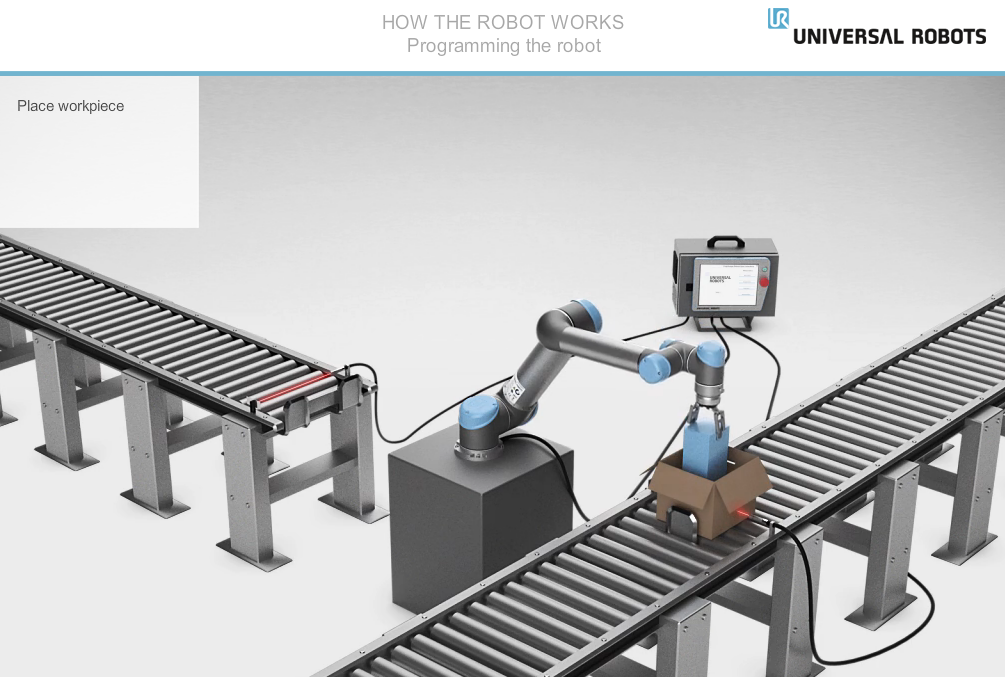
\includegraphics[width=0.85\linewidth]{Images/UR_conveyor}
	\caption[Pick and Place Task]{Universal Robots Pick and Place Task}
	\label{fig:urconveyor}
\end{figure}

To achieve generalization in this project, Reinforcement Learning (RL) together with Image Recognition techniques have been used. This algorithms give the robot the ability of calculating, for each time step, the optimal action to achieve the final goal of picking all the objects from the box and placing them in the objective point. To compute this action the robot needs to gather information about the environment such as its relative position over the box or how the pieces are distributed. This information together is called state, and the robot computes each action depending on it.

To perform this project, a distributed architecture with multiple nodes has been created. Each of them takes care of a different activity. For example, some nodes are used to control the robot, others to gather information about the current state, and others are used to train the Artificial Intelligence algorithm. This architecture has been created using ROS (Robot Operative System) and contributes to the project adding all the advantages of a microservices oriented architecture.

\section{Project Motivation}

The fourth industrial revolution is here, and it will change the way that goods are produced, raising efficiency by increasing the amount of automated processes. 
This will lead to a faster production and a reduction of errors, as machines have the ability to decide and act in fractions of seconds without making mistakes. Furthermore, machines can also be working 24 hours per day stopping just for maintenance checks, which would help to increase the productivity factor without increasing the expense in human resources.

We have been hearing about industry 4.0 since 2011, but the truth is that it is not a reality yet. We are just in the beginning, and it will take decades to perform such a big change in the industry. There are some factors to take in mind in order to analyse the evolution of the industry in the following years. The improvement on the telecommunications with the arrival of 5G networks, the moral dilemma of substituting workers for machines and the impact that this could have in the society or the improvement and implementation of AI technologies are just some of these factors. 

We have seen a lot of Artificial Intelligence algorithms applied to the industry, but the truth is that these technologies are not fully developed yet and just big companies can afford to use them in their supply chain. Besides, there are some task that are now performed by humans and cannot be done by machines due to its complexity or its importance in the whole production chain.

The motivation of this project is to contribute to the industry change providing an open source solution to a complex problem such as disordered pick and place task. This open source solution does not currently exist in the industry and would add value being a good starting point for bigger projects in the future. % Introducción
	\chapter{Description of Technologies}
	Describir las tecnologías, protocolos, herramientas específicas, etc. que se vayan a tratar durante el proyecto para facilitar su lectura y comprensión.
	Hablar de Java no procede aquí porque todo el mundo sabe lo que es, pero si en el proyecto hablo continuamente del protocolo Baseband, debo especificar en este capítulo qué es y para qué sirve.

	\section{ROS + catkin}  % En profundidad
	
		\begin{figure}[h!]
			\centering
			
\includegraphics[width=0.7\linewidth]{Images/logos/ros}
			\label{fig:ros}
		\end{figure}

		
			The first decission we had to make was about the architecture of the project. Was it a good idea to build all the project in the same computer? How should we communicate with the Robot?

		We found the best solution for this questions in ROS (Robot Operative System), which is a framework for the development of software for robots that provides the functionality of an operating system in a heterogeneous cluster. ROS was originally developed in 2007 under the name switchyard by the Stanford Artificial Intelligence Laboratory to support the Stanford Artificial Intelligence Robot (STAIR) project. Since 2008, development has continued primarily at Willow Garage, a robotic research institute with more than twenty institutions collaborating on a federated development model.

		ROS provides the standard services of an operating system such as hardware abstraction, low-level device control, implementation of commonly used functionality, message passing between processes, and package maintenance. It is based on a graph architecture where the processing takes place in the nodes that can receive, send and multiplex messages from sensors, control, states, schedules and actuators, among others. The library is oriented for a UNIX system (Ubuntu (Linux)) although it is also adapting to other operating systems such as Fedora, Mac OS X, Arch, Gentoo, OpenSUSE, Slackware, Debian or Microsoft Windows, considered as 'experimental'.
		ROS is free software under BSD license terms. This license allows freedom for commercial and investigative use. Contributions of packages in ros-pkg are under a variety of different licenses.

		All of these features made ROS ideal for the project. Specially the following ones:
		\begin{itemize}
			\item[\textendash]Universal Robots drivers for ROS using mooveit make it possible to controll ROS remotelly.
			\item[\textendash] ROS is a multi-node oriented framework, which allows us to take all the advantages of micro-services. We can split the software by functionallity gaining:
			\begin{itemize}
				\item[\textendash]The possibility of giving more or less computation power to each functionality depending on its needs. In the project we have useed from  computers with the better Nvidia Graphic card and 32 GB of RAM to other mini-computers such as a Raspberry-pi or an Arduino Card.
				\item[\textendash]The chance of using a different environment for each functionality. Different versions of python and even different programming languages, diferent versions of libraries, diferent Operative Systems, etc.
				\item[\textendash]Isolation of each component of the project, allowing us to develop separatly each functionality without affecting the rest of the functionalities of the project.
			\end{itemize}
			\item[\textendash]It can work over an Arduino Card. It is not self sufficient, as it needs to be serial connected to a computer (Or Raspberry pi) in orther to work. We needed the arduino card in order to build our "home made" vaccuum gripper.
			\item[\textendash]It is open source and have a huge community, so we could reuse some already developed solutions such as the usb\_cam package, which let us take pictures from a camara connected to another node or computer.
			
		\end{itemize}


	\section{pytorch}
	
		\begin{figure}[h!]
			\centering
			
\includegraphics[width=0.7\linewidth]{Images/logos/pytorch}
			\label{fig:pytorch}
		\end{figure}
	
		PyTorch is a Python package designed to perform numerical calculations using tensor programming. It also allows its execution on GPU to speed up calculations.
	
		Typically PyTorch is used both to replace numpy and process calculations on GPUs and for research and development in the field of machine learning, mainly focused on the development of neural networks. In this case we will use PyTorch in both the Reinforcement Learning algorithm and the image Processing.
	
		PyTorch is a very recent library and despite this it has a large number of manuals and tutorials where to find examples. In addition to a community that grows by leaps and bounds.
		
		PyTorch has a very simple interface for creating neural networks despite working directly with tensors without the need for a library at a higher level such as Keras for Theano or Tensorflow.
		
		Unlike other packages like Tensorflow, PyTorch works with dynamic graphs instead of static ones. This means that at runtime the functions can be modified and the calculation of the gradient will vary with them. On the other hand, in Tensorflow we must first define the computation graph and then use the session to calculate the results of the tensors, this makes it difficult to debug the code and makes its implementation more tedious.
		
		PyTorch has support to run on graphics cards (GPU), it uses internally CUDA, an API that connects the CPU with the GPU that has been developed by NVIDIA.

	\section{arduino}
		\begin{figure}[h!]
			\centering
			
\includegraphics[width=0.7\linewidth]{Images/logos/arduino}
			\label{fig:arduino}
		\end{figure}
		Arduino is an open source electronics creation platform, which is based on free hardware and software, flexible and easy to use for creators and developers. This platform allows the creation of different types of single-board microcomputers that can be used by the developer community for different types of use.

		As commented before, we will use Arduino Card in order to build a Vaccuum Gripper for the Robot. It will be connected with all the other nodes using ROS Queues.


	\section{github}
		\begin{figure}[h!]
			\centering
			
\includegraphics[width=0.7\linewidth]{Images/logos/github}
			\label{fig:github}
		\end{figure}
		GitHub, Inc. is a provider of Internet hosting for software development and version control using Git. It offers the distributed version control and source code management (SCM) functionality of Git, plus its own features. It provides access control and several collaboration features such as bug tracking, feature requests, task management, continuous integration and wikis for every project. Headquartered in California, it has been a subsidiary of Microsoft since 2018.
			
		GitHub offers its basic services free of charge. Its more advanced professional and enterprise services are commercial. Free GitHub accounts are commonly used to host open-source projects. As of January 2019, GitHub offers unlimited private repositories to all plans, including free accounts, but allowed only up to three collaborators per repository for free. Starting from April 15, 2020, the free plan allows unlimited collaborators, but restricts private repositories to 2,000 minutes of GitHub Actions per month. As of January 2020, GitHub reports having over 40 million users  and more than 190 million repositories  (including at least 28 million public repositories),  making it the largest host of source code in the world.

	\section{CUDA}
		\begin{figure}[h!]
			\centering
			
\includegraphics[width=0.7\linewidth]{Images/logos/cuda}
			\label{fig:cuda}
		\end{figure}
		CUDA stands for Compute Unified Device Architecture, which refers to a parallel computing platform including a compiler and a set of development tools created by nvidia that allow programmers to use a variation of the language. C programming for encoding algorithms on nvidia GPUs.

		Through wrappers you can use Python, Fortran and Java instead of C / C ++.
		
		Works on all nvidia GPUs from the G8X series onwards, including GeForce, Quadro, ION, and the Tesla line.1 nvidia claims that programs developed for the GeForce 8 series will also work without modification on all future nvidia cards, thanks to binary compatibility.
		
		CUDA tries to exploit the advantages of GPUs over general purpose CPUs by using the parallelism offered by its multiple cores, which allow the launch of a very high number of simultaneous threads. Therefore, if an application is designed using multiple threads that perform independent tasks (which is what GPUs do when processing graphics, their natural task), a GPU will be able to offer great performance in fields that could range from computational biology to biology. crypto, for example.
		
		The first SDK was released in February 2007 initially for Windows, Linux, and later in version 2.0 for Mac OS. It is currently offered for Windows XP / Vista / 7/8/102, for Linux 32/64 bits3 and for macOS4.

	\section{moveit}
		\begin{figure}[h!]
			\centering
			
\includegraphics[width=0.7\linewidth]{Images/logos/moveit}
			\label{fig:moveit}
		\end{figure}
	
		MoveIt! is open source software for ROS (Robot Operating System) which is state of the art software for mobile manipulation. In fact, we could say that MoveIt! it is becoming a de facto standard in the field of mobile robotics, as today more than 65 robots use this software, including the latest robots developed by Robotnik.
		
		MoveIt! includes various utilities that speed up the work with robotic arms, and it helps to not be continually “reinventing the wheel”, following the ROS philosophy of code reuse.
		
	\section{Universal Robots driver for ROS}	
		\begin{figure}[h!]
			\centering
			
\includegraphics[width=0.7\linewidth]{Images/logos/ur}
			\label{fig:ur}
		\end{figure}
	
	
		Universal Robots have become a dominant supplier of lightweight, robotic manipulators for industry, as well as for scientific research and education. The Robot Operating System (ROS) has developed from a community-centered movement to a mature framework and quasi standard, providing a rich set of powerful tools for robot engineers and researchers, working in many different domains.
		
		With the release of UR’s new e-Series, the demand for a ROS driver that supports the new manipulators and the newest ROS releases and paradigms like ROS-control has increased further. The goal of this driver is to provide a stable and sustainable interface between UR robots and ROS that strongly benefit all parties.
	
	
	\section{UR3 robot}
	
		% TODO: Definir el número de motores independientes del robot y los tipos de coordenadas y movimientos que se pueden hacer con él
	
		The UR3 Universal Robots robot is the smallest cobot of the UR series of Universal. Universal Robots' ultra flexible UR3 provides high precision for the smallest production environments.
		
		\begin{figure}[h!]
			\centering
			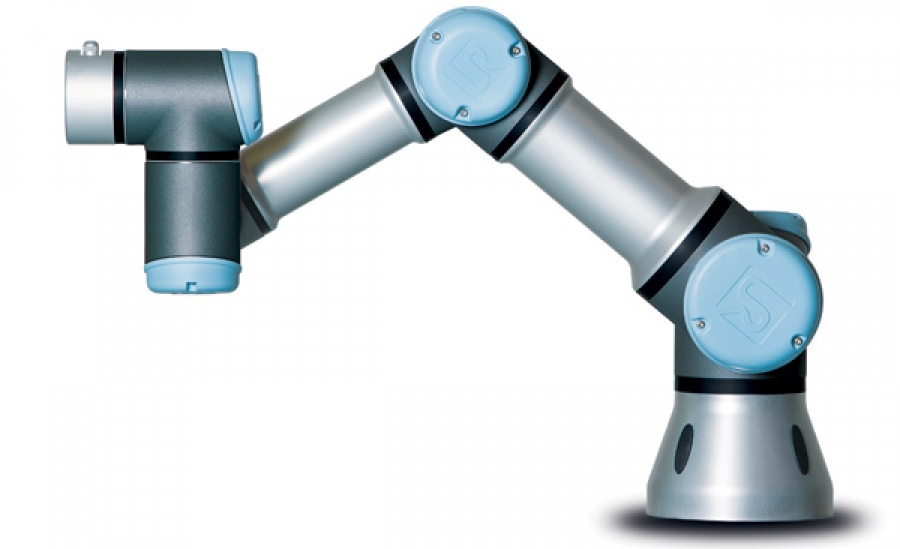
\includegraphics[width=0.7\linewidth]{Images/logos/ur3}
			\label{fig:ur3}
		\end{figure}
	
		
		It can modulate payloads of up to 3 kg, adding value to scientific, pharmaceutical, agricultural, electronic and technological facilities. Tasks the UR3 excels at include: mounting small objects, gluing, screwing, tool handling, welding and painting.
		
		However, the range of movements of this robot is really limited, and it can only lift up 3 Kilograms so this robot is really good for preparing a prototype, it has the same characteristics than its big brothers, but probably it is not good enough to build a production solution.	
		
	\section{anaconda}
		\begin{figure}[h!]
			\centering
			
\includegraphics[width=0.7\linewidth]{Images/logos/anaconda}
			\label{fig:anaconda}
		\end{figure}
		Anaconda is a free and open distribution of the Python and R languages, used in data science, and machine learning. This includes processing of large volumes of information, predictive analytics and scientific computations. It is aimed at simplifying the deployment and management of software packages.
		
		The different versions of the packages are managed through the conda package management system, which makes it quite easy to install, run, and update data science and machine learning software such as Scikit-team, TensorFlow and SciPy.
		
		The Anaconda distribution is used by 6 million users and includes more than 250 data science packages valid for Windows, Linux, and MacOS.

	
 % Description of Technologies
	\chapter{State of the art}
	
	The pick and place task that is intended to be performed in this thesis is really useful for a lot of applications into the industrial world because it would bring a lot of flexibility for these processes. A example of this applications could be an assembly line, where robotic arms could be picking all the different pieces to assemble in the product using always the same algorithm.
	
	Big companies are developing a lot of Artificial intelligence use cases in the industry, and they try to contribute to the AI community by publishing scientific articles on how they managed to use AI for their specific tasks. Unfortunately, although some companies have already developed their own solutions for our specific pick and place task, none of them have published a scientific article on the subject, making it difficult to study the way they have achieved it.
	
	One of the companies that has already developed a pick and place task is the Japanese automation company Fanuc, which has developed an AI-based solution together with Preferred Networks. As commented before, they have not published any scientific article about the topic but we can see the system working in a video they have posted on YouTube \cite{preferred_networks_inc_bin-picking_2015}. That means that we have to gather all the possible information from the video, where we could find that they have not used a Reinforcement Learning algorithm but just a Deep Neural Network (DNN) with image recognition. 
	
	To train the net, they have collected "success" or "fail" labelled images by making pick actions in random places of the box. Once they gathered a big enough dataset of images, they have trained a Deep Neural Network as the one we see in \autoref{fig:fanucdnn}, where we can also see that the Neural Net has been trained to predict whether the robot is going to success in a pick action in a specific place or not. Using that net, they can make a heat map of the whole box, predicting the points of maximum probabilities of succeed. As usually, they noticed that the bigger the image dataset, the higher the success ratio. In eight hours, they reach 90\% of success, which they say is bigger than the human success ratio.
	
	\begin{figure}
		\centering
		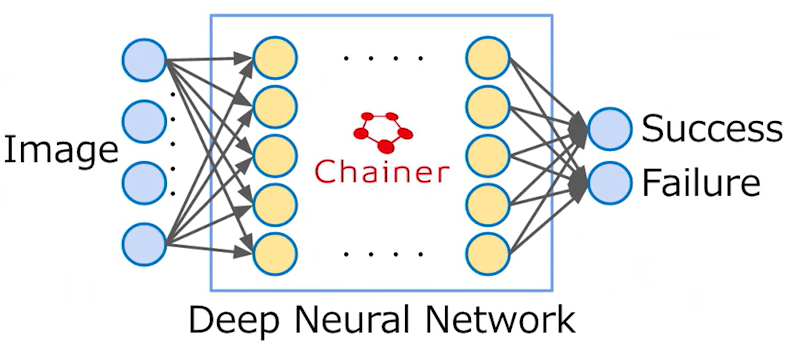
\includegraphics[width=0.85\linewidth]{Images/FANUC_DNN.png}
		\caption[Fanuc DNN]{Deep Neural Network of Fanuc solution (taken from the video)}
		\label{fig:fanucdnn}
	\end{figure}
	
	\subsection{Reinforcement Learning}
	
		The idea of the project is to keep using image recognition techniques but, in our case, applied to a \textbf{Reinforcement Learning} Algorithm which is an area of machine learning inspired by psychology behavioural. Its goal is to determine what actions a software agent should choose in a given environment in order to maximize some notion of "reward" or accumulated prize. 
		
		Explained easily, RL is used to make an \textbf{agent} (the robot) learn how to interact with a \textbf{environment} in order to perform a task. To achieve this, Markov Decision Process (MDP) which provides a mathematical framework for modeling decision making in situations where outcomes are partly random and partly under the control of a decision maker.
		
		\subsubsection{Markov Decision Process (MD)}
			In MDP, the environment is what we are actually trying to simulate with the MDP. The agent will interact with it to learn how to perform the task, so these are the attributes of the environment:
			\begin{itemize}
				\item[\textendash]\textbf{Agent:} The agent is the most important piece of the algorithm because it represents the objects that we want to become smarter.
				\item[\textendash]\textbf{Actions (A):} The agent can interact with the environment by performing a set of actions which is normally finite.
				\item[\textendash]\textbf{States (S): } Each time the agent performs an action, it moves to a new state. States are basically the set of information that differentiates the situation of the agent before and after performing an action. States can be transitional or terminal, when the agent meets the objective or when it gets to a forbidden position.
				\item[\textendash]\textbf{Rewards (R):} Each time an action is performed, the agent receives a reward. This reward can be positive, negative or null depending on the impact of the action to achieve the objective.
				\item[\textendash]\textbf{Policy ($\pi$):} The policy is used to define the optimal action for each step. It gives a punctuation for all of the actions in the current step as shown in the following formula. The agent takes the action with highest punctuation.
				\begin{gather*}
					\pi(a|s)=P_r\{A_t=a|S_t=s\}
				\end{gather*}
			
			\end{itemize}
			
			The MDP is divided in discrete timesteps (t), where each timestep does not have to last the same time as the previous step. Each timestep, the agent uses the policy $\pi$ to decide the next action. 
			
			Once the action is taken:
			\begin{itemize}
				\item[\textendash]The environment transits to th next state: \textbf{ \boldmath$S_t = S_{t+1}$}.
				\item[\textendash] Environment produces a new reward, which can be represented with the following formula: \boldmath
				\begin{gather*}
					P(s', r, s, a) = P_{r}\{S_{t+1}=s', R_t=r, S_{t}=s, A_{t}=a\}
				\end{gather*}
			\end{itemize}
			
			Agent's performance is calculated in terms of its future accumulated rewards known as return. This is called \textbf{expected return} an is calculated as  shown in the formula below, where $\gamma$ is the discount factor, and is used to give a bigger value to the closest steps.
			
			\begin{gather*}
				G_t = \sum_{k=t} \gamma ^{k-t} \cdot R_{k+1} \:\: \forall \:\: \gamma \in [0, 1]
			\end{gather*}
		
		
		\subsubsection{Q-Learning}
			
			Now that we know all these concepts, we have to learn what Reinforcement Learning Algorithms do to learn. Basically, \textbf{the goal of the agent is to find a policy that maximizes the expected return }. This can be done using different strategies as:
			\begin{itemize}
				\item[\textendash]\textbf{Q-Learning:} Estimating action values using Q Tables or other methods
				\item[\textendash]\textbf{TRPO:} Parametrizing the policy and optimizing its parameters
			\end{itemize}
			
			Basic Q-Learning is based on the assumption that both actions and states are limited and that the same action in the same state always drives to the same new state. Having this in mind, Q-learning algorithms build two matrices of shape \textbf{length(actions) x length(states)} as shown in the \autoref{fig:q-matrix}.
			
			\begin{figure}[h]
				\centering
				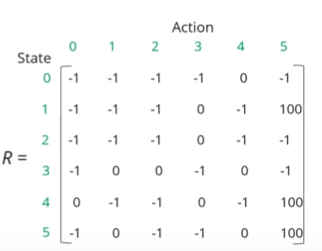
\includegraphics[width=0.7\linewidth]{Images/Q-Matrix}
				\caption[Q-Matrix]{Reward and Q Matrix shape in Basic Reinforcement Learning}
				\label{fig:q-matrix}
			\end{figure}
			
			In these two matrices, Q-Learning algorithm stores in the R matrix the reward for the pair of action-state while in the Q matrix they store cumulated reward for this same pair. The Q matrix is the one used to decide which action to perform in each state and R matrix the one used to calculate the reward of each action. 
			
			However, for the aim of this project, the states of the agent can be different in each timestep. The state would actually be partially formed by images, so the number of states can be infinite. We need a more complex version of Reinforcement Learning.
			
	\subsection{Deep Reinforcement Learning}
		
		The approach of mixing both image recognition and RL is called Deep Q Learning (DQN) or Double Deep Q Learning (DDQN) depending on the implementation and uses Neural Networks in two different stages of the algorithm. Firstly, a Convolutional Neural Network (CNN) is used to extract image features, and then, a Deep Neural Network (DNN) is used to calculate the q value of each independent action and select the next one using these values.
		
		DQL was proposed in 2012, and, since then, it has been used for a lot of different purposes. For example, Guillaume Lample and Devendra Singh Chaplot demonstrated back in 2017 that a RL agent could play FPS Games using as inputs just game scores and pixels from the screen \cite{lample_playing_2018}. Another really interesting example is this robot \cite{zhu_target-driven_2017}, which is capable of moving around a house looking for an objective and avoiding obstacles using DDQL.
		
		A good resource to understand how Reinforcement Learning really works is Deeplizard's tutorial \cite{noauthor_reinforcement_nodate}. In this tutorial they explain different versions of the algorithm and how to implement them in python to solve different OpenAI gym environments \cite{openai_gym_nodate}. 
		
		Deep Reinforcement Learning is though an union between RL and image recognition, but let's see how it actually works. The main idea is to replace the Q-table that we saw before for a Dense Neural Network that uses as input another Neural Network, a Convolutional Neural Network (CNN). The full algorithm would have as many outputs as allowed actions. Therefore, simplifying, these outputs re equivalent to the q-values saw before and so we will call them. To see it graphically, when the agent wanted to take an action, he  would pass the state image through the Neural network represented in \autoref{fig:deepqnetwork} and would take the action with higher q-value.
		
		\begin{figure}[h]
			\centering
			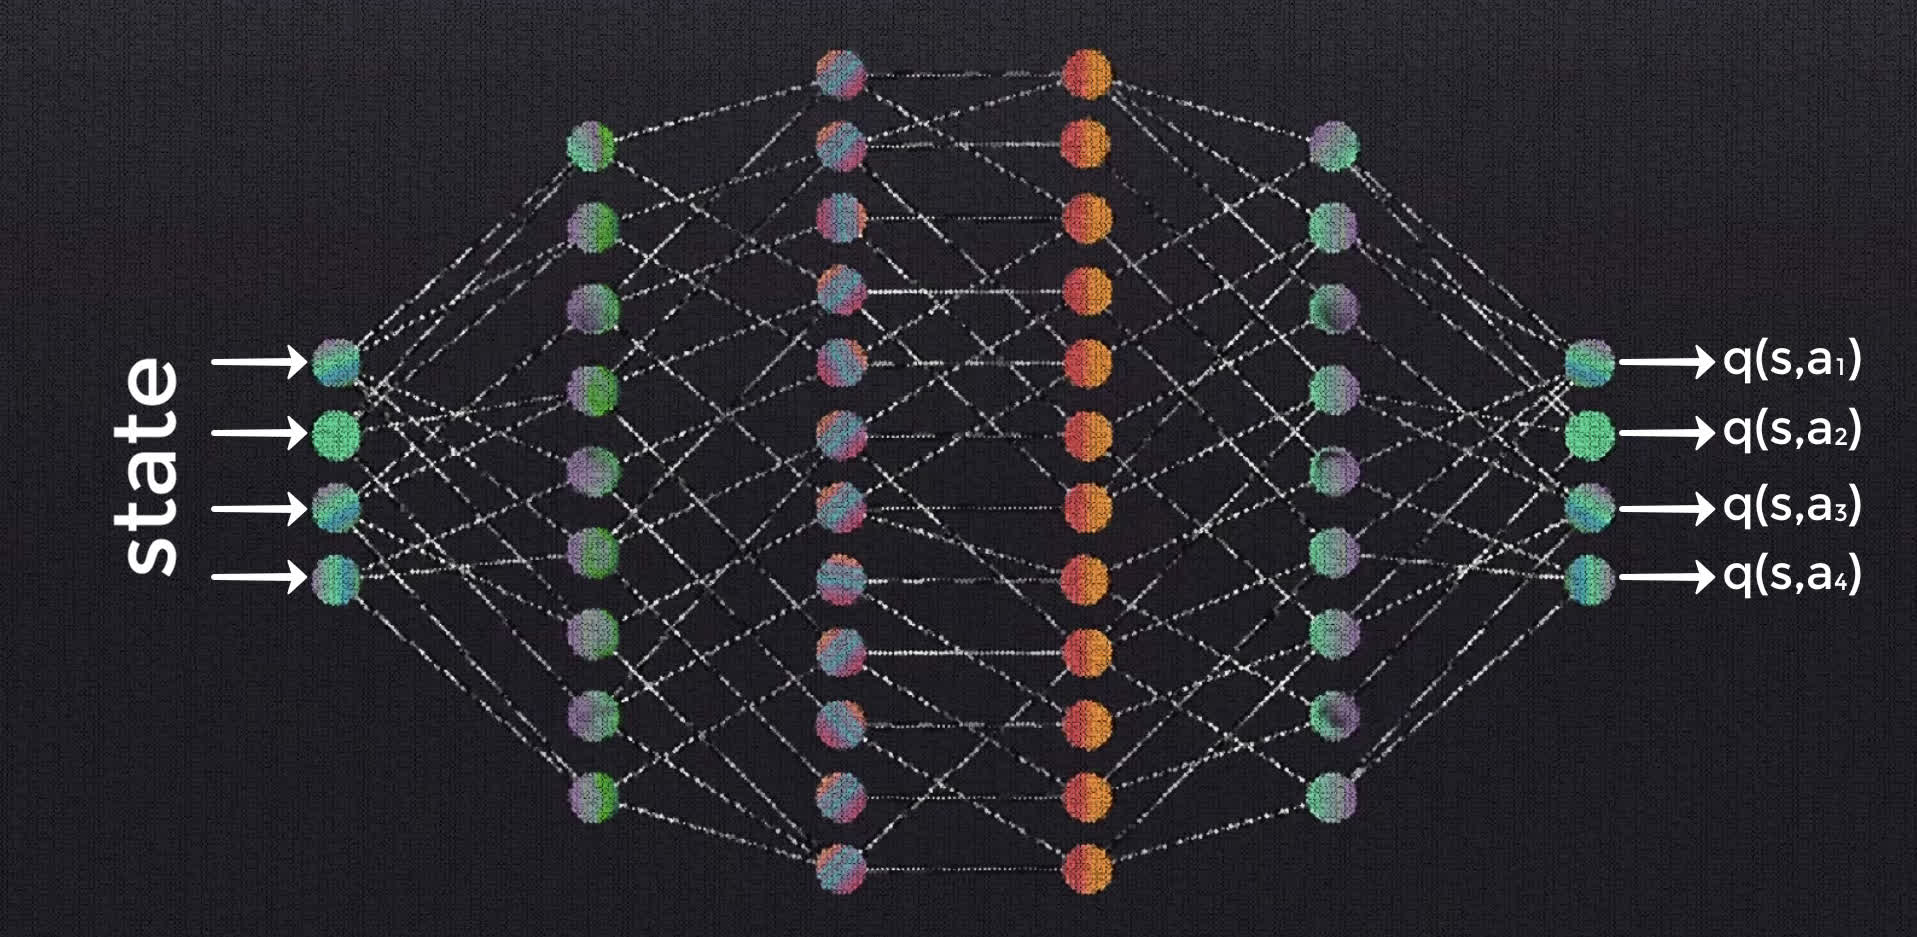
\includegraphics[width=0.7\linewidth]{Images/DeepQ-Network.jpg}
			\caption[Deep Q Learning]{Deep Q Learning Representation with 4 outputs}
			\label{fig:deepqnetwork}
		\end{figure}
		
		When I said "simplifying" in the previous paragraph, I meant "simplifying a lot" in the next paragraphs I will explain all the intermediate steps in the algorithm and why they are important:
		
		\begin{itemize}
			\item[\textendash]Episodes and Steps
			\item[\textendash]Exploration vs Exploitation trade-off
			\item[\textendash]Replay Memory
			\item[\textendash]Bellman's Equation
			\item[\textendash]Target and Policy Networks
		\end{itemize}
	
		\subsubsection{Episodes and Steps}
			RL training is divided in Episodes. One Episode is the sequence of actions needed to reach a terminal State. Each time the agent reaches a terminal state, an episode is ended, and a new one is started.
			
			On the other hand, steps represents every time that a new action is taken, so the number of steps taken by the agent during training is infinite. Later on, we will use as metric of performance the number of steps per episode, as they must decrease during the training.
		
		\subsubsection{Exploration vs Exploitation trade-off}
			In Reinforcement Learning there are two important concepts that are \textbf{Explore} and \textbf{Exploit}. To explore is basically gather new information about the environment and to exploit is to make the best decision with the information that we already have.
			
			In Deep Reinforcement Learning, the agent exploit the information gathered by using the pre-trained Neural Network to decide next action. On the other hand, the agent explore the environment by deciding next action randomly. We use exploration mainly in the beginning of the training because we want the agent to gather as much information of the environment as possible before starting training.
			
			When the agent uses exploitation, it is also gathering information about the environment. However, we could not let the agent explore this way because during the exploration phase we want all the actions to be performed with the same probability and neural network bias can cause some actions to be performed much more than others.
			
			So, how do we decide when the agent must explore or exploit? To decide it we can use multiple techniques, but the most common one is the Epsilon-Greedy Strategy. This strategy basically consist on setting a probability of exploring and keep decreasing it slowly during the training. It works this way:
			
			\textbf{\begin{enumerate}
				\item We set the initial exploring probability ($\epsilon$)
				\item We set the per-step epsilon decay, ($\epsilon\_decay$)
				\item For each step:
				\begin{enumerate}
					\item With probability $p = \epsilon$, the agent explores the environment (takes a random action). If not, it exploit the information by deciding the action using the NN.
					\item Whether the agent has explore or not, we decrease the probability of exploring the environment in the next step ($\epsilon = \epsilon - \epsilon\_decay$)
				\end{enumerate}
			\end{enumerate}}
			
			Using this strategy, the agent will rather explore or exploit the environment during the training. In the first steps the probability of a random action (exploring) will be much hihger than in the last steps of the algorithm. This probability will keep decreasing during the training, until it reaches the minimum exploring rate, which is normally set to 10%.
			
		
		\subsubsection{Replay Memory}
		
			Every time that the agent performs an action, either by exploring or exploiting, the agent lives an experience. For the purpose of training the algorithm, we will store all these experiences.
			
			Experiences are formed by the initial state, the action taken, the state reached (final state) and the reward gotten and they are stored in the Replay Memory. Then, every time that an action is taken, the algorithm is trained following this steps:
			
			\begin{enumerate}
				\item Replay Memory checks if the number of experiences is higher than the batch size
				\item If there are enough experiences:
				\begin{enumerate}
					\item Replay Memory supplies a random set of experiences of size=batch\_size.
					\item With this set of experiences, the target network is trained.
				\end{enumerate}
			\end{enumerate}
			
			Optimizing Replay Memory can be a challenge, because, if we are using a Graphic Card in the training, we would be storing all the experiences in its memory. But, why do we need to store all the experiences? We could also be using the last N experiences to train the network and it would be a less memory-consumption demanding solution. 
			
			The answer to this question is that Reinforcement Learning Networks converge really slowly and variance between consecutive steps is really low. Using consecutive experiences to train the network would result though in a slower and biased learning. Besides, this way of working is better for learning real-world experience, where there are infinite different states, as the experience gained in previous steps will be used multiple times later to train the network.		


		\subsubsection{Bellman's Equation}
			As commented before, Deep Reinforcement Learning uses Neural Networks to compute the q-values of each action. The optimal value of these q-values is represented by the Bellman's Equation and is shown below:
			
			\begin{gather*}
				q_*(s,a) = E[ R_t + \gamma max(q_*(s', a' )]
			\end{gather*}
			
			As we can see in the equation, the optimal value depends in both the reward of the action taken and the maximum optimal q-value of the next action. In real life it is impossible to compute this value, because we would be an infinite loop. However, as the most important parameter of the formula is the expected reward ($q_*(s', a' )$ is multiplied by the discount factor $\gamma$), we can simply use the next action q-value and it will be a good approximation. The formula would stay as follows:
			
			\begin{gather*}
				q_*(s,a) = E[ R_t + \gamma max(q(s', a' )]
			\end{gather*}
		
			With this new formula we will be able to compute the optimal q-value for each experience stored in the Replay Memory (initial state, action, final state and reward). It is important to have in mind for this process that the optimal q-value can only be computed if the action has actually been taken, because we don't know the Reward of non taken actions. But, anyway, why do we need to compute the optimal q-value?
			
			To answer this question, lets take a look to the training process of the neural network:
			
			\begin{enumerate}
				\item the agent decide which action to take using the policy-network. (action with highest q-value)
				\item The agent takes the action and receives a reward from the environment
				\item The agent stores all the experience in the Replay Memory
				\item The training process is started:
				\begin{enumerate}
					\item A random batch of experiences is taken from the Replay Memory
					\item For all these experiences, its optimal q-value is calculates using the modified Bellman's Equation and target-network
					\item For all these experiences, the actual q-value is calculated using the policy-network
					\item For all these experiences, the loss is calculated as the difference of both values
					\item We use the Neural network optimizer to back-propagate the loss to all the weights
				\end{enumerate}
			\end{enumerate}
		
			So, to answer the previous question, we need to compute the\textbf{ optimal q-values in order to calculate the loss} of the neural network for each action taken and train, though, the algorithm.
			
			Retaking here the question answered before about why we needed Replay Memory module, one important reason is that one action taken in the initial steps of the training will affect differently to the neural network in this moment than later, when the network is already trained, and its q-value is though more similar to the optimal q-value. Replay Memory technique allow us to use this information gathered in any step of the training, during a step where the network is more trained.
			
		
		\subsubsection{Target and Policy Networks}
			In the previous step, we talk about two different networks: policy and target. The target network comes to solve a stability problem of the DRL training. In the next paragraphs I will explain the problem and how target network can help to solve it.
			
			Having in mind the way we calculate the loss of the neural network in the previous section we can realize that we have to pass information through the network twice. Just to remember:
			
			\begin{gather*}
				loss = R_t + \gamma max(q(s_{t+1}, a_{t+1})) - q(s_t, a_t)
			\end{gather*}
		
			As a spoiler, I can say that $q(s_{t+1}$ and $q(s_t, a_t)$ will not be calculated with the same network. But.. why?
			
			Imagine that we have an experience, which is composed of an initial state, an action that has been taken, the state reached with this action and a reward. Remembering previous section, the loss of the neural network is calculated as the difference between the q-value of the initial state and the action taken and the optimal q-value of the expected cumulative reward (or target value) of the action.
			
			Q-values are calculated using the states as input of Neural Networks. Let's see what could happen if we calculated both of the values with the same network. In this case, once we had the loss calculated, we would use back-propagation to adapt the weights of the Neural Network and make the q-value of the initial state more similar to the target q-value.
			
			The problem here comes because as both q-values are using the same Neural network to be calculated, when we change the weights to move the initial q-value to one direction, the target q-value is moving in the same direction, so we have not reduce the distance between the two values. It is basically like a dog chasing its tail.
			
			To solve this problem we introduce the target-network. This network is basically a frozen clone of the policy network that we only use to calculate the target value of each action. This way, when we gain stability during the training of the RL Algorithm. The target-network is updated periodically after a certain amount of steps, so is always updated.
			
			
		\subsubsection{DQL Training}
			
			During the previous sections I have been explaining a lot of concepts about Deep Reinforcement Learning Training. I have explained them and how they affect the training. It is a really complex process so probably a sum-up will help understanding it.
		
			The training basically uses the following schema:
			
			\begin{itemize}
				\item[\textendash]Initialize replay memory capacity.
				\item[\textendash]Initialize the policy network with random weights.
				\item[\textendash]Clone the policy network, and call it the target network.
				\item[\textendash]For each episode:
				\begin{itemize}
					\item[\textendash]Initialize the starting state.
					\item[\textendash]For each time step:
					\begin{itemize}
						\item[\textendash]Select an action via exploration or exploitation
						\item[\textendash]Execute selected action and observe reward and next state.
						\item[\textendash]Store experience in replay memory.
						\item[\textendash]Sample random batch from replay memory.
						\item[\textendash]Preprocess states from batch.
						\item[\textendash]Pass batch of preprocessed states to policy network.
						\item[\textendash]NN training. Weight back-propagation:
						\begin{itemize}
							\item[\textendash]Calculate loss between output Q-values and target Q-values.
							\item[\textendash]Using both the target and the policy networks to increase stability.
							\item[\textendash]Gradient descent updates weights in the policy network to minimize loss.
						\end{itemize}
						
					\end{itemize}
				\end{itemize}
				\item[\textendash]After X time steps or episodes, weights in the target network are updated to the weights in the policy network.
			\end{itemize}
			
			This training can also be explained with \autocite{fig:training}, where the Pool is the Replay Memory that stores the sample (experiences) from real interaction with the environment and feeds the training node of random sample of experiences.
			
			Then, we can see that we use the Q-Network (policy network) to predict actions, but also to calculate the q-value of Replay Memory's batch. Then, we use the target network to predict action-value of state s1 with the predicted action in Q estimation Network, andthis network is updated in a low rate.
			
			Finally, the action taken in the Dynamic Environment can be predicted by the Neural Network or Randomly chosen (Stochastic search). This is the way of representing epsiolon-Greedy Strategy. 
			
			\begin{figure}
				\centering
				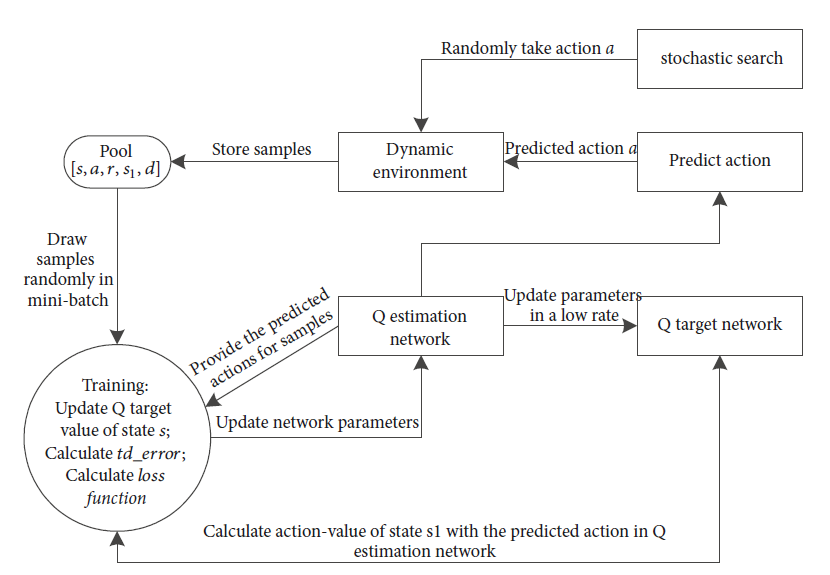
\includegraphics[width=0.7\linewidth]{Images/Training}
				\caption[RL Training]{Reinforcement Learning Training Summary}
				\label{fig:training}
			\end{figure}
				
			
		
		
	\subsection{Problems of Deep Reinforcement Learning in Real-world}
		
		Real-world problems introduces some challenges that we will have to manage. In march 2018, A. Rupam Mahmood, Dmytro Korenkevych, Brent J. Komer, and James Bergstra explained the problems they found while implementing a RL algorithm in a UR5 robotic arm \cite{mahmood_setting_2018}.
		
		Some of the problems they found were the following:
		
		\begin{itemize}
			\item[\textendash]Slow rate of data-collection, as movements in the real robot are slower than in a simulated environment. 
			\item[\textendash]Partial observability. Sensors cannot retrieve all the information about the environment.
			\item[\textendash]Noisy sensors will provide inaccurate information.
			\item[\textendash]Safety of the robot and its surroundings have to be taken in mind.			
			\item[\textendash]Fragility of robot components.
			\item[\textendash]Delay between an action is requested and the time it is actually performed can affect the training.
			\item[\textendash]Preparing the robot is a really difficult task:			
			\begin{itemize}
				\item[\textendash] Controlling the robot.
				\item[\textendash] Define all aspects of the environment.
				\item[\textendash] Difficulties for obtaining random and independent state when episode ends.
			\end{itemize}
		\end{itemize}
		
		Another problem that can be found in our project is that, as objects are randomly placed, the environment that the agent will have to face will be completely different each time. In fact, the robot can interact with the environment, as it can move the pieces trying to pick them, so we are facing a dynamic environment RL problem. A good example of a dynamic environment problem is the path planning of a self driven car, where each time the agent takes an action the environment will change and, furthermore, obstacles do not have to be static, but they can also move.
		
		%% TODO: Explicar en profundidad (En descripción de las tecnologías)
		There are multiple examples of articles on this topic, such as the one Xiaoyun Lei, Zhian Zhang, and Peifang Dong published in September 2018 using a DDQN approach to solve it \cite{lei_dynamic_2018}. However, there are other solutions as the one proposed by Marco A. Wiering \cite{wiering_reinforcement_2001}, where he introduces some prior knowledge to the model in order to facilitate the learning. His algorithm had problems generalizing the environment, so he introduced some prior information about the model together with a Model-based RL. This made the algorithm more capable to learn without loosing a lot of trainable capability.
		
		%% The task they performed is really different from the one we are implementing, but, as they are using the same robot, most of the problems they found are valid for our project. The solution for these problems will be explained later.
		
		%% TODO: Comentar más artículos de investigación
 % State of the art
	\chapter{Definition of the Project}

	\section{Motivation}
		The project motivation is the natural continuation of a previous project performed at ICAM University. This project was part of the assembly line of a car manufacturing process and its objective was to pick some specific plastic pieces and place them into the product. To achieve this, the system used opencv image processing, so it was recognising a specific shape given apriori.
		
		This project was totally functional and the robot could perform the task with a high successful rate. However, the lack of generalization of the system makes it hard to introduce changes as using it for another part of the assembly line. Each time that this happened someone would have to introduce the shape of the pieces to the system and to calibrate the camera to the new environment. 
		
		The motivation of the project is to create from scratch a new solution for performing the picking of the pieces. This time, the project will not be sponsored by any company, so there will be less resources to use.
		
		With this new approach, the idea is to use all the knowledge of previous documented projects on Artificial Intelligence in the industry and make a little contribution to the huge advance of industry 4.0. In fact, the idea is to make the project completely replicable so that anyone could use this project as a starting point for new applications.

	\section{Objectives}
		\todo{Revisar objetivos y adaptarlos al proyecto}
		The objectives of the project are five and are listed and explained below:
		
		\begin{itemize}
			\item[\textendash]Implement a bin picking simple solution. A basic one, without Artificial Intelligence.
			\item[\textendash]Improve the performance using RL and Image Recognition.
			\item[\textendash]Study the usage of new technologies to add information to the system. Adding physics or new image recognition techniques.
			\item[\textendash]Test different tools such as Multiflash or 3D images to improve performance.
			\item[\textendash]Add value to the scientific community making the solution available if the previous objectives are reached.
		\end{itemize}
	
	\section{Methodology}
		This project will be performed using an agile methodology, which is one of the simplest and effective processes to turn a vision for a business need into software solutions. Agile is a term used to describe software development approaches that employ continual planning, learning, improvement, team collaboration, evolutionary development, and early delivery. It encourages flexible responses to change \cite{noauthor_agile_nodate}.
		
		In the case of this project, the team is just formed by two workers and a project manager. This make necessary to make some changes to the typical agile methodology. For example, daily meetings are substituted by constant communication between both workers and weekly meetings with the project director. With this approach, all the members of the project are updated about how it is going and have clear objectives.
		
		Likewise, the methodology of this project is based in three fundamental principles as it is shown in \autoref{fig:methodology}. The first two principles are highly related, as the project is iterative because it is experimental. That means that the way of working is perform little sprints with new functionalities, test them (experimental) and, depending on the results, define the new sprint, execute it and test again (iterative). Besides, the project is also incremental because the idea is starting implementing the simplest possible solution and keep adding new improvements to it in a iterative loop until the optimal configuration is reached.
		
		\begin{figure}
			\centering
			
\includegraphics[width=0.85\linewidth]{Images/methodology}
			\caption[Methodology]{Methodology}
			\label{fig:methodology}
		\end{figure}
		
	
	\section{Planning and budget}
	
			Regarding the planning, there are some really important functionalities that have been defined since the beginning of the project, as they are needed. These functionalities are split in three different groups: Hardware implementation, Artificial Intelligence Implementation and Robot controller implementation. The tasks related to these three groups are shown in \autoref{fig:planning1}, \autoref{fig:planning2} and \autoref{fig:planning3}. 
		
		\begin{figure}
			\centering
			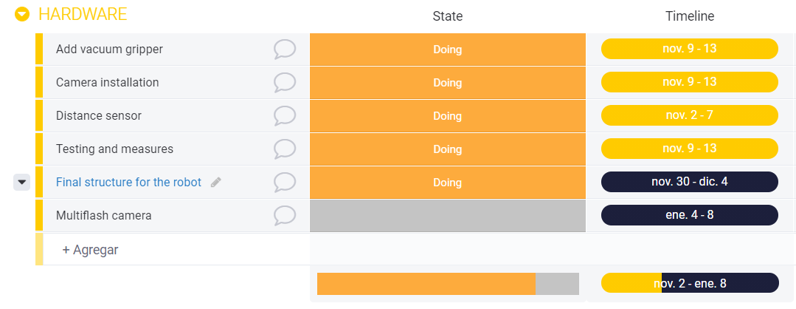
\includegraphics[width=0.85\linewidth]{Images/planning1}
			\caption[Chronograph HW]{Chronograph of the Hardward implementation}
			\label{fig:planning1}
		\end{figure}
		
		
		\begin{figure}
			\centering
			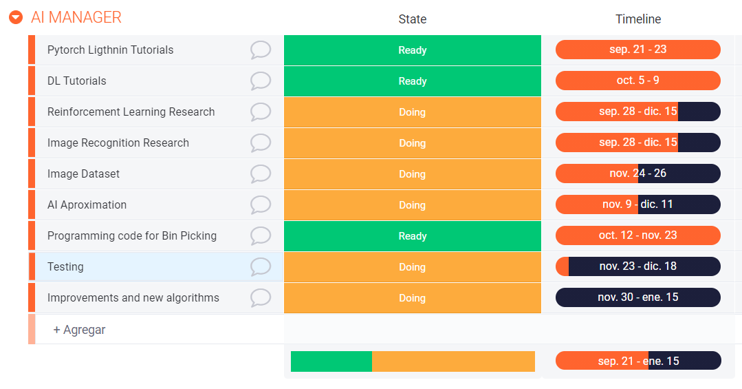
\includegraphics[width=0.85\linewidth]{Images/planning2}
			\caption[Planning AI]{Planning of the Artificial Intelligence implementation}
			\label{fig:planning2}
		\end{figure}
		
		
		\begin{figure}
			\centering
			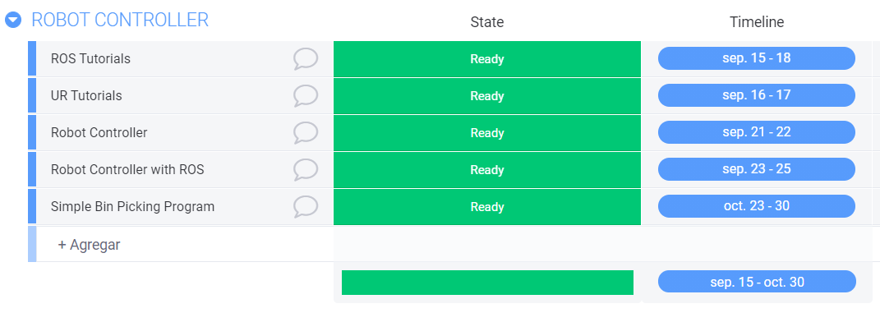
\includegraphics[width=0.85\linewidth]{Images/planning3}
			\caption[Planing Robot Controller]{Planning of the Robot Controller implementation}
			\label{fig:planning3}
		\end{figure}
		
		\todo{Añadir presupuesto} % Definition of the Project
	\chapter{Developed System}

	In previous sections of this documents, I have explained the main idea of the project, and what technologies are going to be used to develop a fully functional system. Just to remember, the objective of the project is to perform a Pick and Place task using a Universal Robots' UR3 robotical arm.
	
	The objects have to be taken from a box (Environment Box) and placed in another box (Place box). The pieces had to be something light due to the limitations of the UR3 robot that we commented before. As there wasn't any sponsor for the project we could decide the shape of the pieces, and we decided to use 5 cm size wooden squares as the ones showed in \autoref{fig:pieces}.
	
	\begin{figure}[h]
		\centering
		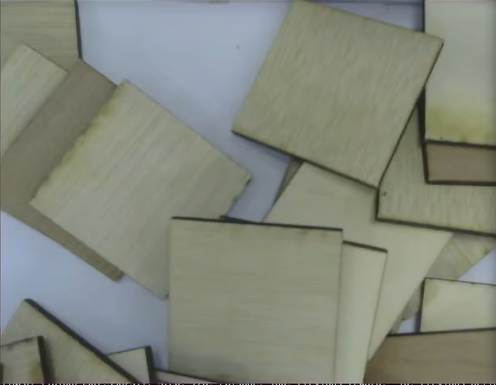
\includegraphics[width=0.7\linewidth]{Images/pieces}
		\caption[pieces]{Wooden Pieces used in the project}
		\label{fig:pieces}
	\end{figure}
	
	\section{Hardware Architecture}
	
		In order to make this system work, we need a really complex architecture that can be split in three different categories. These categories are:
		
		\begin{itemize}
			\item[\textendash]Environment
			\item[\textendash]sensorimotor devices
			\item[\textendash]Computational devices
		\end{itemize}
	
		To understand it better, we are going to use \autoref{fig:imagen-arquitectura} and \autoref{fig:imagen-arquitectura-ii}, which are labeled pictures of the architecture, where we are going to be able to see how the components of the architecture are like. 
		
		\begin{figure}[H]
			\centering
			\includegraphics[width=0.9\linewidth]{"Images/Imagen Arquitectura"}
			\caption[Picture of Architecture I]{Labelled picture of the Architecture I}
			\label{fig:imagen-arquitectura}
		\end{figure}
	
		
		\begin{figure}[H]
			\centering
			\includegraphics[width=0.9\linewidth]{"Images/Imagen Arquitectura II"}
			\caption[Picture of Architecture II]{Labelled picture of the Architecture II}
			\label{fig:imagen-arquitectura-ii}
		\end{figure}
	
		In the pictures we can see multiple elements tagged with different colours and labels. Each colour represents a category. 
		
		
		The environment elements, that can be found in green, and labelled with EN, are basically all the things that the robot will have to interact with. The sensorimotor elements, that can be found in orange and with the label SM, are all the elements needed to allow the robot interact with the environment. And finally, in blue and with label CP, we can find the computational elements, which are the ones used to receive all the sensor information, decide which movement to do, and communicate with the robot and the gripper for them to actually perform these actions.
		
		But, what are all these elements? Let's explain them:
		
		\begin{itemize}
			\item[\textendash]\textbf{Environment}: We can see this elements in both images, from different perspective.
			\begin{itemize}
				\item[\textendash]\textbf{EN1}: The Environment box where the agent has to take the pieces
				\item[\textendash]\textbf{EN2}: The box where the agent has to place the pieces
			\end{itemize}
			\item[\textendash]\textbf{Sensorimotor devices} Ones are showed in one image, and others in the other.
			\begin{itemize}
				\item[\textendash]\textbf{SM1}: This is the Onboard camera, used for the agent to decide which action to take. It is attached to the gripper, so in the picture they are shown together.
				\item[\textendash]\textbf{SM2}: Together with the camera, we can see the "Home made" gripper used to pick the pieces.
				\item[\textendash]\textbf{SM3}: the upper camera, where the agent can pick a global picture of the environment. This picture will be important, but we will explain it later.
				\item[\textendash]\textbf{SM4}: the pump of the Gripper.
				\item[\textendash]\textbf{SM5}: Both 12V and 24V power adaptor used to feed the pump and some sensors.
			\end{itemize}
			\item[\textendash]\textbf{Computational devices}. In the picture we cannot see all the computer used in the project, but there are 2 icons used to represent  them.
			\begin{itemize}
				\item[\textendash]\textbf{CP1}: This is the ROS Master Node. All of the nodes of the system will be connected to this node. Besides being the master node, robot\_controller node and Universal Robots driver will also bo running in this computer.
				\item[\textendash]\textbf{CP2}: This computer is a really powerful one, with one of the bes graphical cards in the market an 32 GB of RAM. It will be used to train the algorithm, running the ai\_manager node.
				\item[\textendash]\textbf{CP3}: This mini-computer can be seen in one of the pictures and its a Raspberry-pi. This computer will be used as a bridge form the arduino card of the gripper and the ROS master node. The cameras will also be attached to the Raspberry-pi.
			\end{itemize}
		\end{itemize}
	
	\section{Logical Architecture}
		
		Once we have seen the physical architecture of the project, let's see how the Software architecture is. The Logical architecture will use all the elements commented on the previous section, and they will work together using ROS (Robot Operative System). 
		
		\begin{figure}
			\centering
			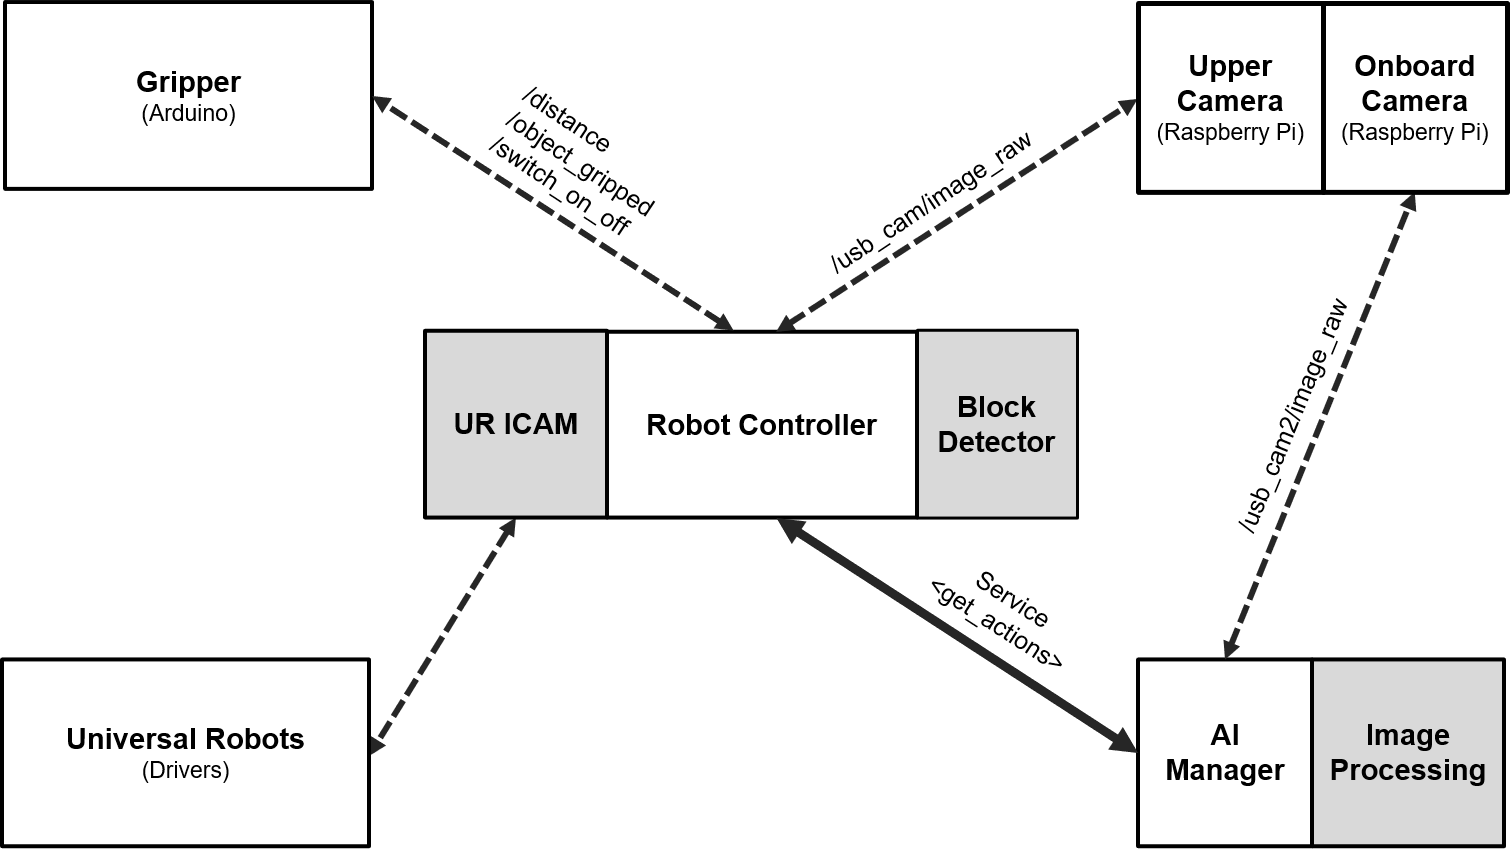
\includegraphics[width=0.7\linewidth]{Images/Architecture}
			\caption[Logical Architecture]{Logical Architecture of the project}
			\label{fig:architecture}
		\end{figure}
	
		In \autoref{fig:architecture} we can see the logical architecture of the application, which is composed of 6 nodes communicating one with each other. We can see that the communication topics are written in the figure and that there are some squares attached one to another, and some of them are grey. All the white squares are ROS nodes, while grey ones are separate pieces of code that the nodes are using, but they are not ROS nodes by themselves. On the other hand, both camera nodes that are together in the upper right corner are two independent nodes, but using the same code to send the cameras images.
		
		To explain briefly what every node does, probably it is easier going step by step from the simplest architecture to the final one, so that we see what every node is doing.
		
		\begin{figure}[H]
			\centering
			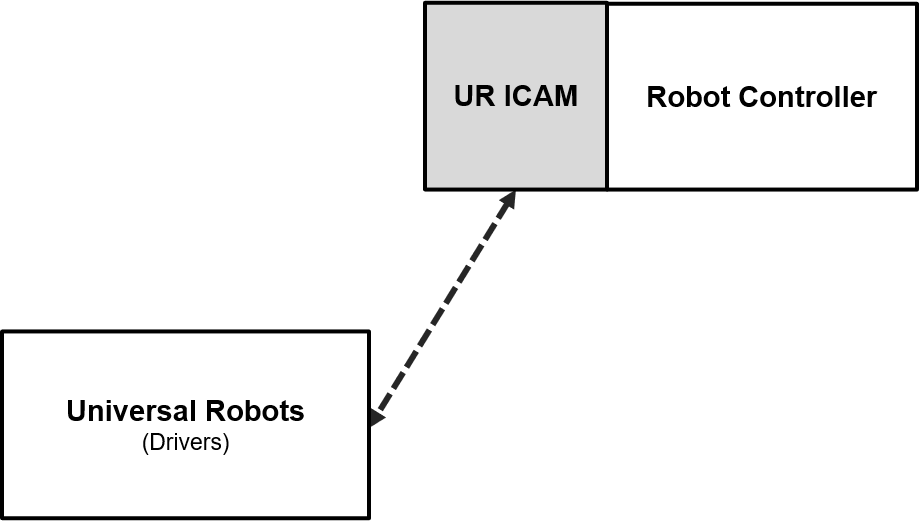
\includegraphics[width=0.7\linewidth]{Images/ArchitectureI}
			\caption[Architecture I]{From the simplest to the final Architecture I}
			\label{fig:architecturei}
		\end{figure}
	
		In \autoref{fig:architecturei}, there are only three components. However, Both Universal Robots Drivers and UR ICAM were not developed by us and are like black-boxes for us. That is the reason why there are no ROS topics written in the communication the figure.
		
		Universal Robot Drivers is the one that actually communicates with the robot, and provides all the basic tools needed to control it remotely. On the other side, UR ICAM node is a node developed in the university, and it provides us some methods to control easier the robot. These methods are a personalization of the ones provided by MoveIt library, and they make us possible to go to some angular coordinates of the robot without calculating the optimal path to reach this position, or the same thing with some cartesian coordinates.
		
		Finally, the Robot Controller node is the one that actually is communicating with all the othe nodes of the architecture. All the actions that the robot will be able to perform are here, so just with Robot Controller node we could almost be able to implement a silly random agent to perform a pick and place task.
	
		\begin{figure}[H]
			\centering
			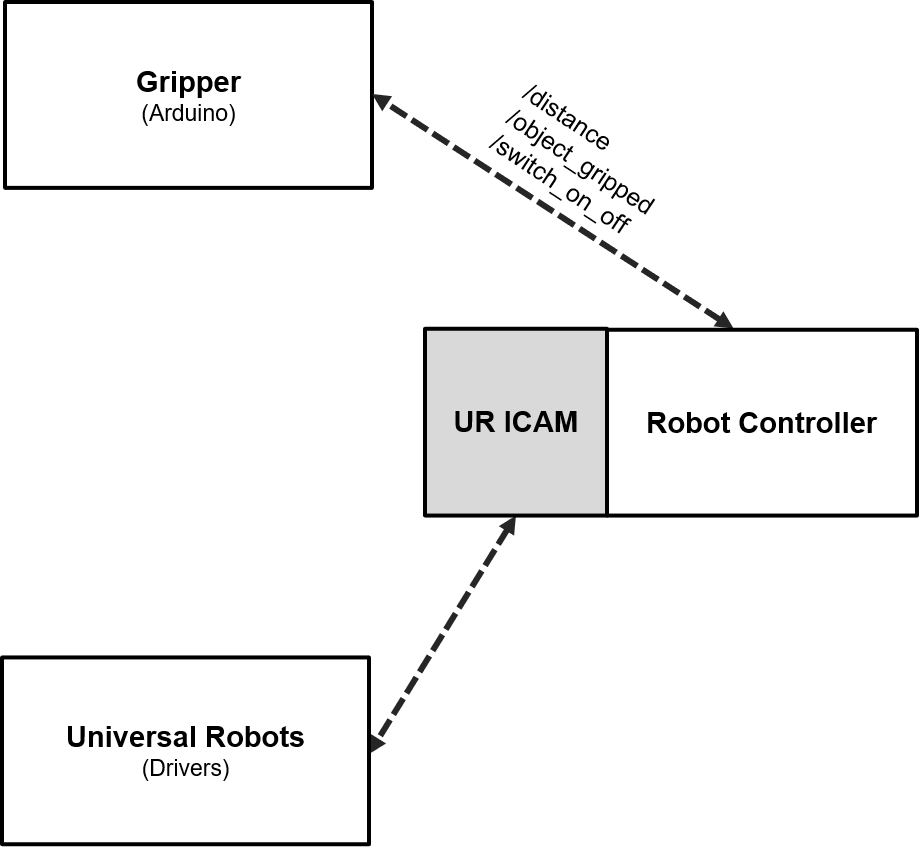
\includegraphics[width=0.7\linewidth]{Images/ArchitectureII}
			\caption[Architecture II]{From the simplest to the final Architecture II}
			\label{fig:architectureii}
		\end{figure}
	
		I said almost, because to perform a pick and place task we also need the gripper node, as we can see in \autoref{fig:architectureii}. This node is running in an ardunio carda communicates by serial port with a Raspberry Pi, which is also connected with the master node. The gripper node uses 3 different topics to communicate with Robot Controller:
		
		\begin{itemize}
			\item[\textendash]\textbf{\textit{\textbackslash distance: }} The gripper is publishing continuously if the gripper is being pushed up or not. Robot Controller wants this information to know when to stop during the pick movement. The Robot basically goes down while \textbf{\textit{\textbackslash distance}} are "False" and stops when they are "True".
			\item[\textendash]\textbf{\textit{\textbackslash switch\_on\_off: }} The gripper listens to this topic. When it receives a "True" message it switch the gripper on, and when it receives a "False" message it switch the gripper off.
			\item[\textendash]\textbf{\textit{\textbackslash object\_gripped: }} The gripper is publishing continuously if there is an object gripped or not. Robot Controller use this information during the pick action. When this action is finished, robot controller checks if an object has been picked or not by reading from this topic. If an object has been picked it goes to the box to place the object and, if not, it just finishes the pick action and request AI Manager for a new action.
		\end{itemize}
	
		\begin{figure}[H]
			\centering
			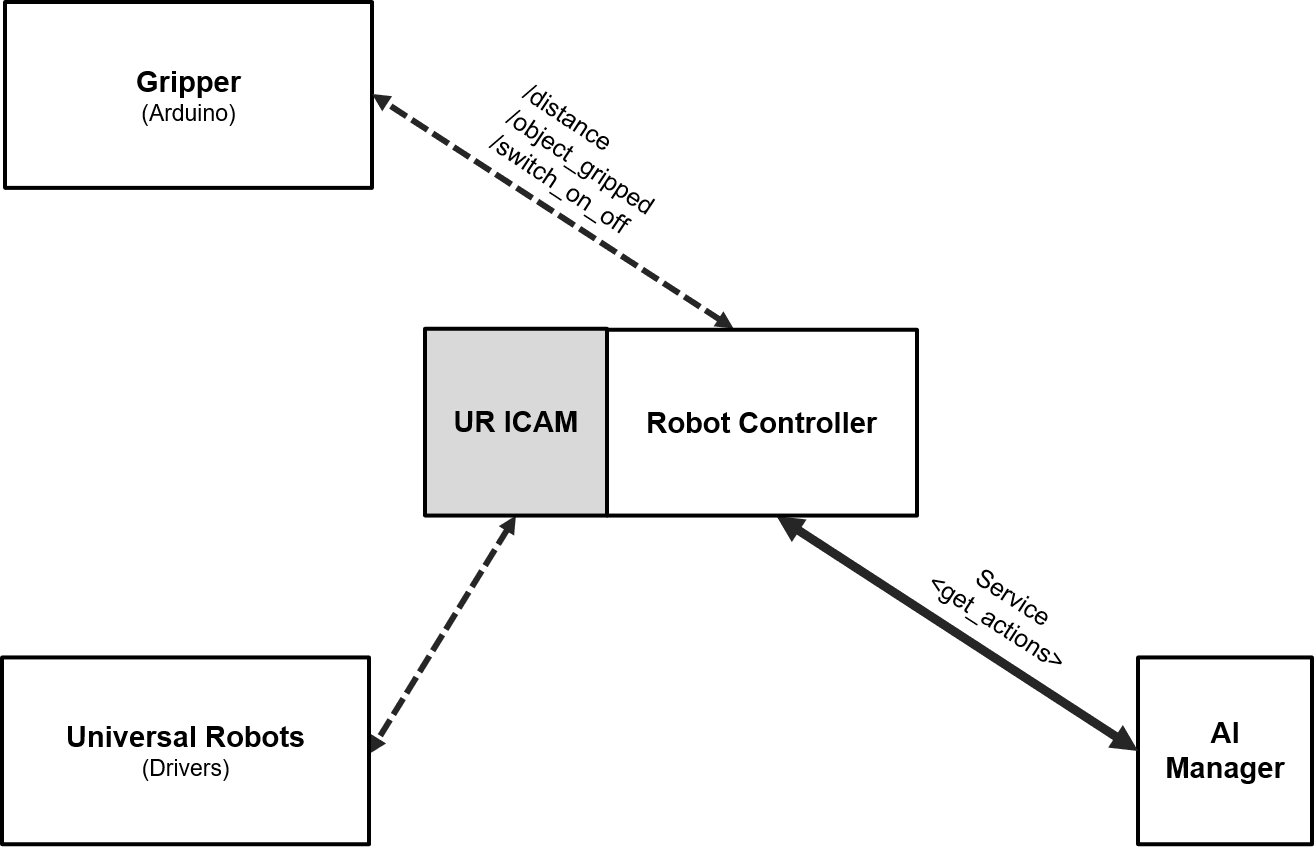
\includegraphics[width=0.7\linewidth]{Images/ArchitectureIII}
			\caption[Architecture III]{From the simplest to the final Architecture III}
			\label{fig:architectureiii}
		\end{figure}
	
		The next step in our trip would be adding the AI Manager Node. This Node is the one who decides which action to perform in each time step. It receives the Coordinate, request an image of the environment (Which in this step is still simulated) and trains a Reinforcement Learning Algorithm to decide which action to perform in each step.		
		
		As we can see in the \autoref{fig:architectureiii}, the arrow representing the communication between Robot Controller and AI Manager is the only continuous line. This is because the communication method is different, in this case we are using ROS Services instead of publishing the messages in topics.
		
		In ROS, the most common way of communicating is using ROS Messages. ROS Messages are simple data structures that are send to a topic, which is basically a queue stored in the Master node. Then, other nodes can be subscribed to this topics so every time that they are free, they ask the master node about the unread messages in the topic. This is called asynchronous communication and, it is probably the best way of sending messages between nodes, because it allows the receiver to adapt its computational needs to the message load received from the topics.
		
		However, in this case asynchronous communication was not possible, because ROS Messages does not ensure the delivery. This was a problem because the Robot Controller could request an action to the AI Manager, and the second one could not receive the message. This is not a problem in this direction because we can solve it by putting a timeout in Robot Controller, and it could make a new request after x time. 
		
		Anyway, this could not be a solution because we need to avoid the AI Manager node to receive the same request twice. This is needed because every time that the AI Manager receives a new action, a new step of the training is performed: A reward is given, random probability decreases, Experience is saved, etc.
		
		ROS Services is the way of performing synchronous communication in ROS, and it ensures that every message is delivered once and only once. AI Manager is though a resting node that does nothing until the Robot Controller nod request an action. It then start calculating the action, trains the net and return the selected action.
		
		get\_actions services is defined by two structures:
		
		\begin{itemize}
			\item[\textendash]Request structure:
			\begin{itemize}
				\item[\textendash]\textbf{x\_coordinate:} X coordinate of the robot used to calculate the reward and training the robot.
				\item[\textendash]\textbf{y\_coordinate:} X coordinate of the robot used to calculate the reward and training the robot.
				\item[\textendash]\textbf{object\_gripped:} Boolean telling whether the robot has an object gripped or not. It is used to calculate the reward of pick actions.
			\end{itemize}
			\item[\textendash]Response structure:
			\begin{itemize}
				\item[\textendash]String telling the action selected
			\end{itemize}
		\end{itemize}
	
		\begin{figure}[H]
			\centering
			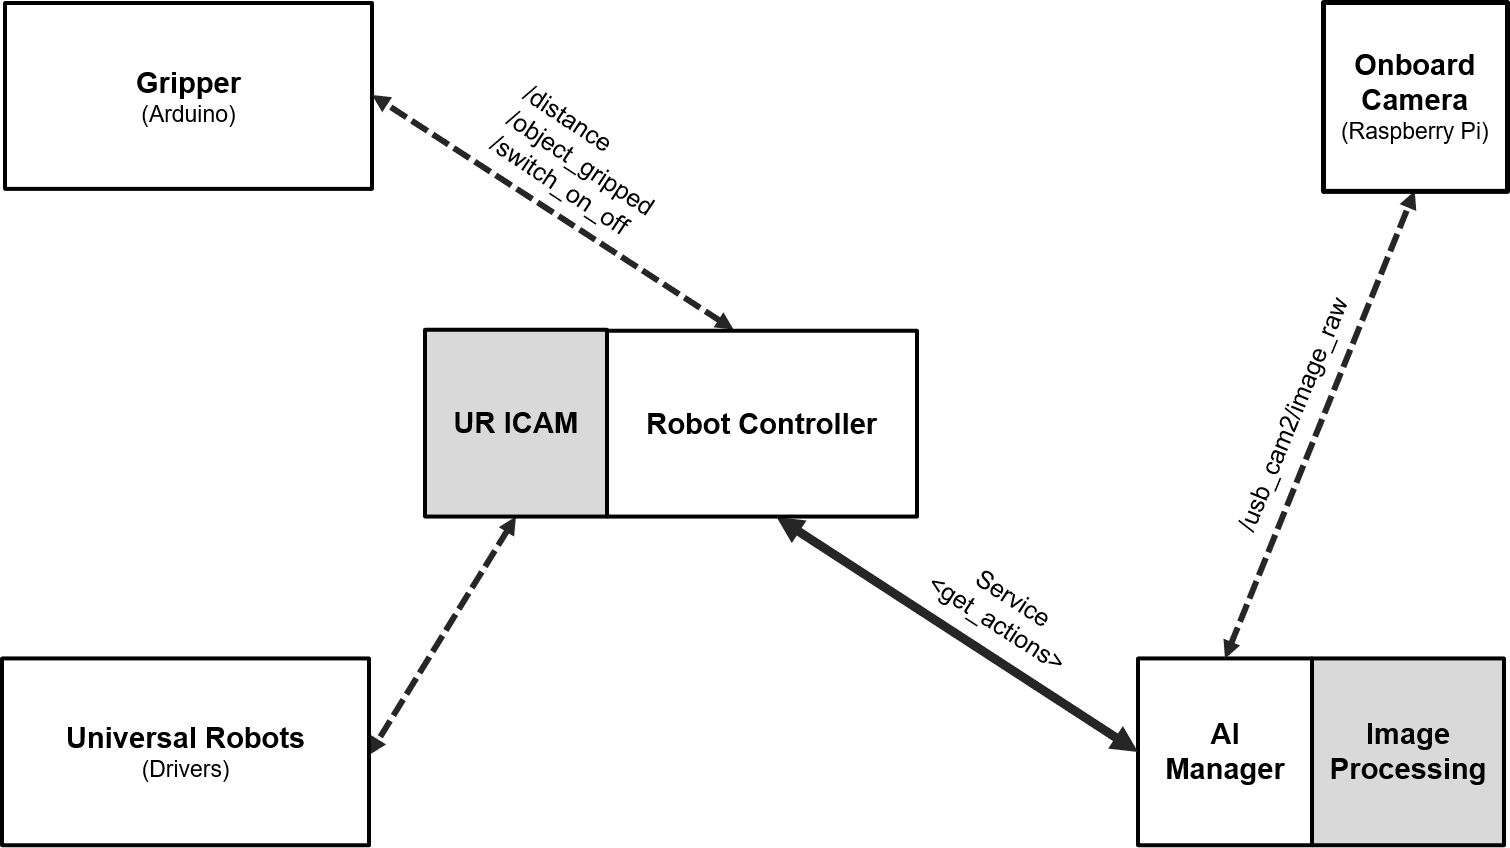
\includegraphics[width=0.7\linewidth]{Images/ArchitectureIV}
			\caption[Architecture IV]{From the simplest to the final Architecture IV}
			\label{fig:architectureiV}
		\end{figure}
	
		We commented before that AI Manager needs to gather a state image in order to start the training. To gather this image, it just requests a message from \textbf{\textendash \textit{usb\_cam\textendash image\_raw}} topic. Messages of this topic are published by Onboard Camera node, which is basically an instance of usb\_cam node that publishes with a 30 fps rate the images of the Onboard camera of the robot. 
		
		But once the Ai Manager has the image, it has to process it and extract its features, and Ai Manager will do it using the models in Image Processing. We will talk deeply about this later, but it basically means to make some transformation to the image (Changing its shape, color, rotation, etc. ) and pass it through a pre-trained Convolutional Neural Network in order to extract some features. This features are actually the ones that will be passed through the Reinforcement Learning Neural Network and the ones that will be stored in the Replay Memory.
		
		Finally, the last two nodes that we have not commented from \autoref{fig:architecture} are the Block Detector and the Upper Camera Node. Block Detector is a piece of code used by Robot Controller when it is performing a place action. In this moment, the robot is out of the box and has to decide the initial coordinates of the next episode. The upper camera has, though, a full view of the environment, so the Robot Controller takes the environment picture from the topic \textbf{\textendash \textit{usb\_cam2\textendash image\_raw}} where the Upper Camera node is publishing the images of the upper camera. Then it passes the image to the Block Detector which finally calculates the optimal point of return, avoiding the places of the box where there are no pieces.
		
		\begin{figure}[H]
			\centering
			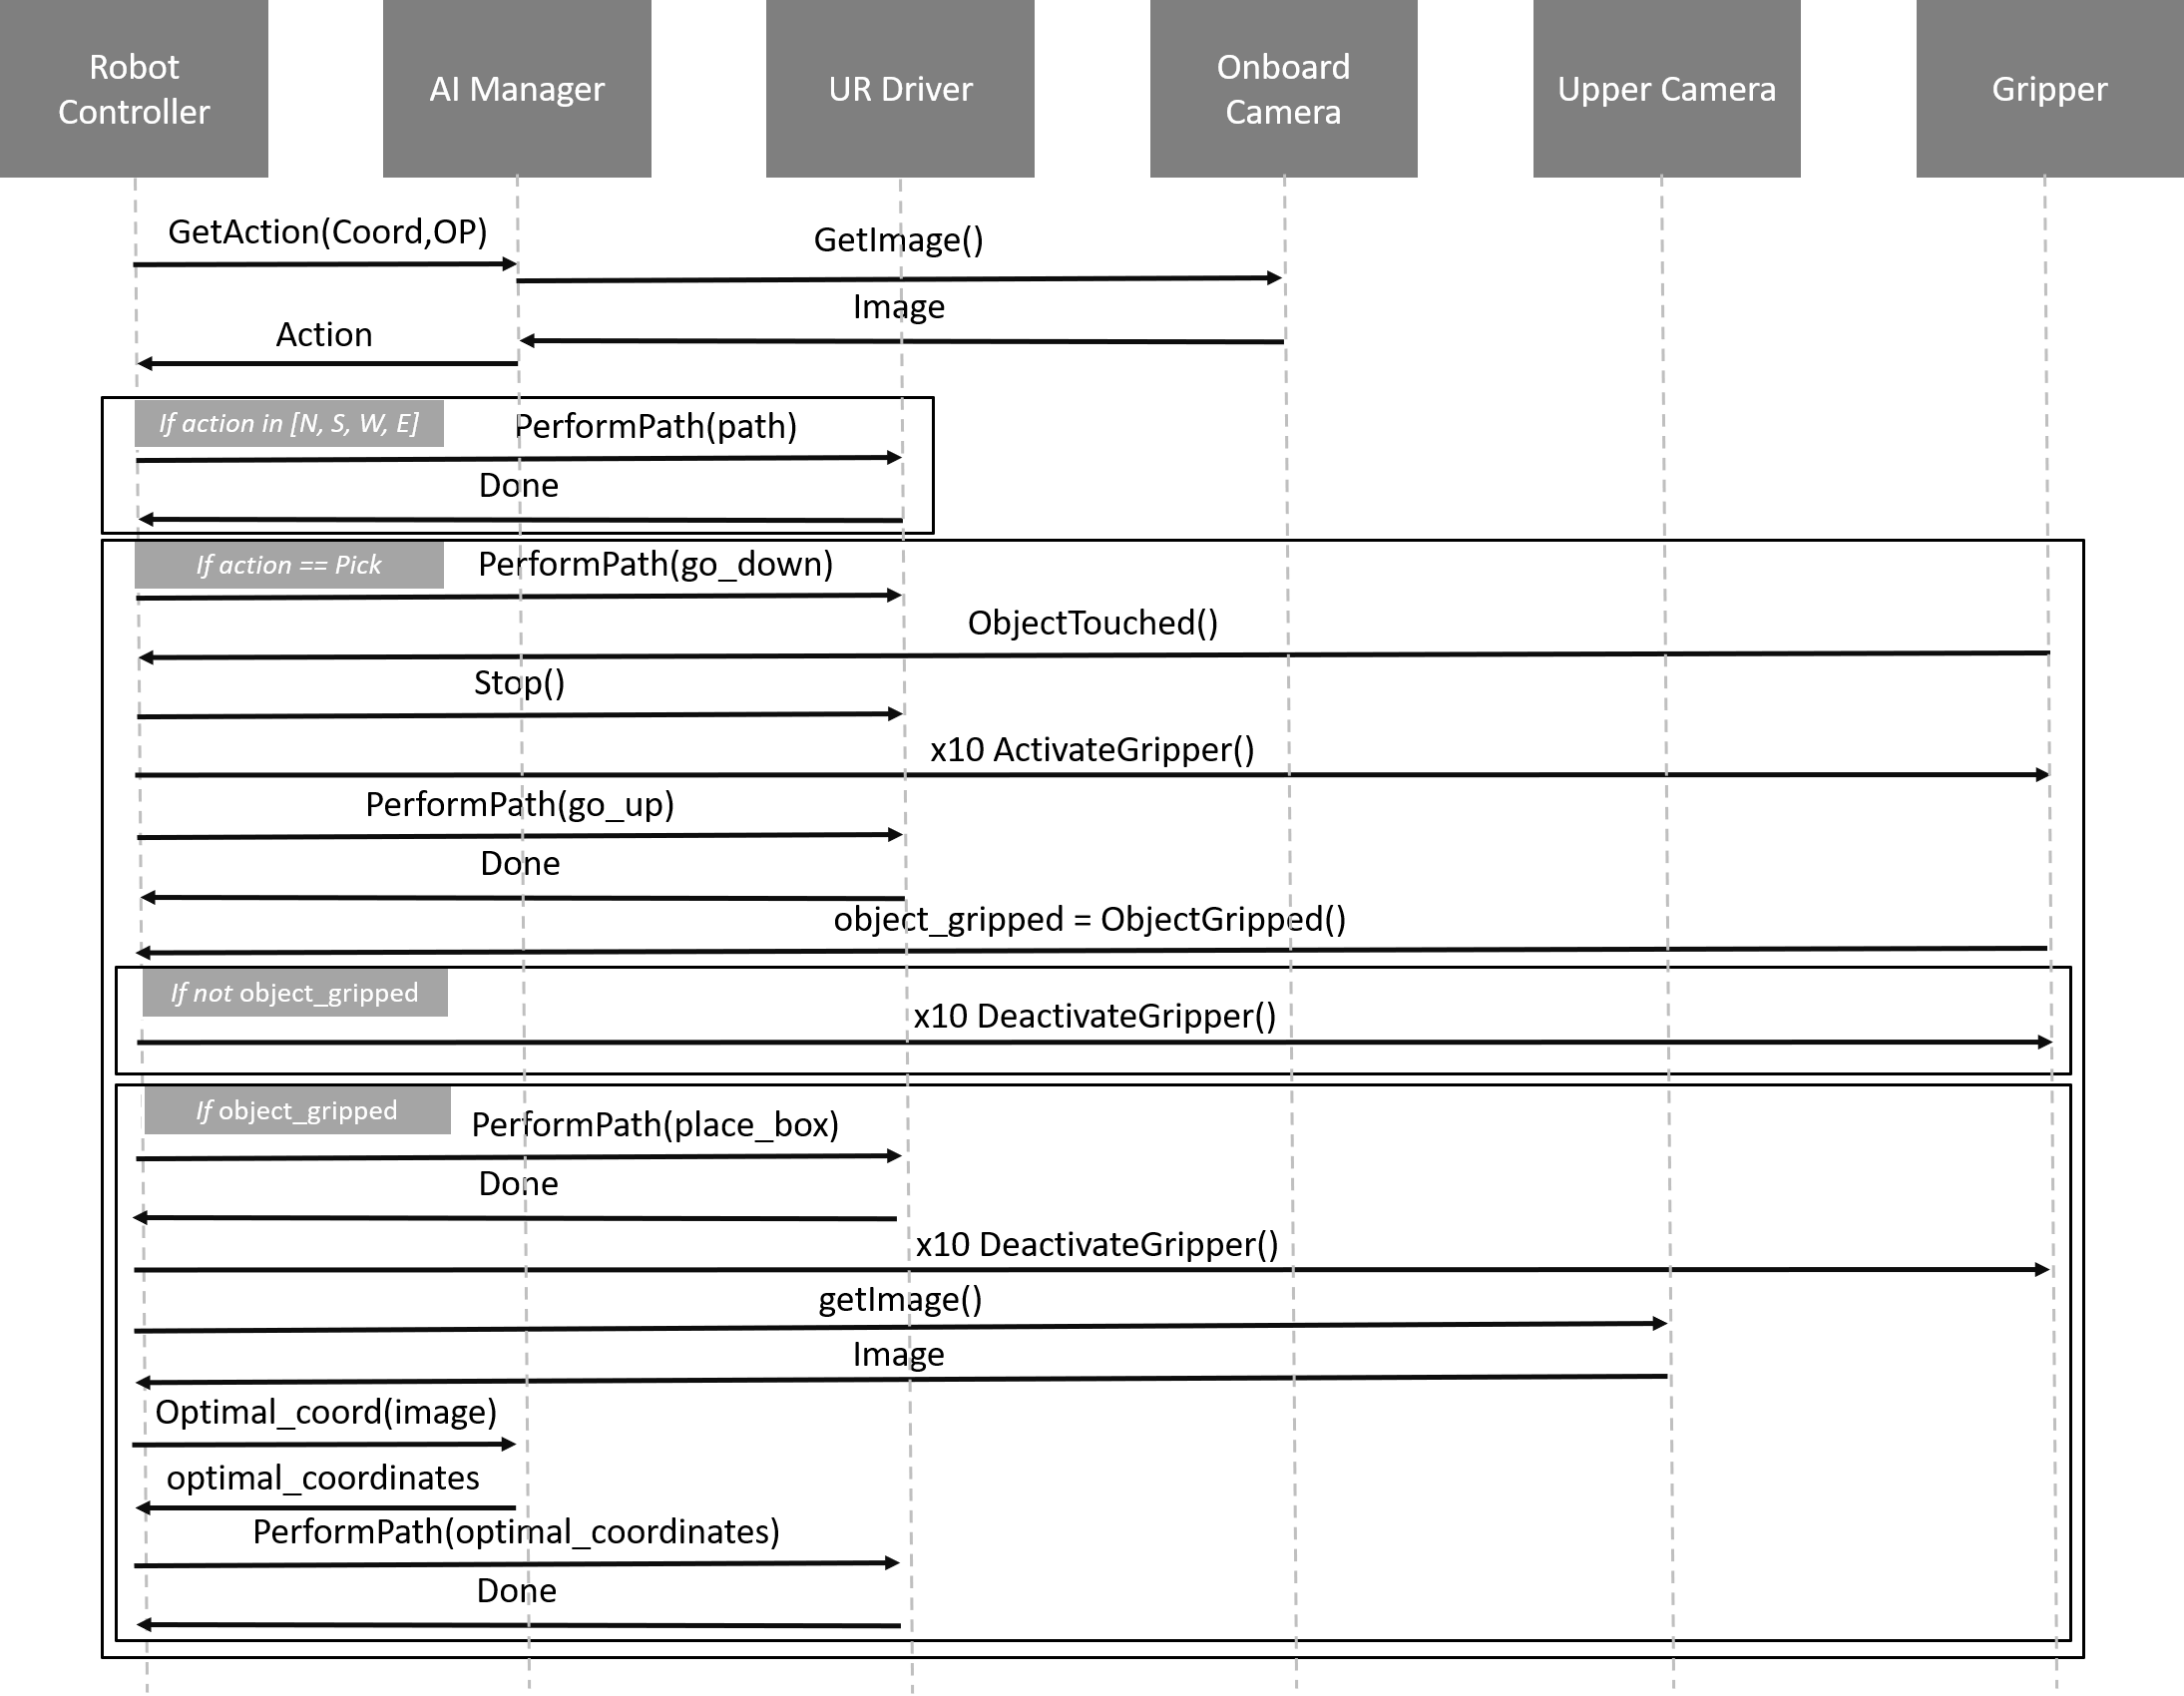
\includegraphics[width=1\linewidth]{Images/NodeInteraction}
			\caption[Node Interction]{Flow Chart of nodes interacting}
			\label{fig:nodeinteraction}
		\end{figure}
	
		To understand better all the architecture, in \autoref{fig:nodeinteraction} we can find a flow chart showing the iteration between nodes in one step. This flow would be in an infinite loop until the training is over. We can see how the step always starts with Robot Controller Asking AI Manager which action to perform, and AI Manager retrieving a picture from Onboard Camera to decide the action and train the Reinforcement Learning Algorithm. Behind this steps there is a complex process that we will talk about later.
		
		Then, depending on the action to perform, the flow would be really simple or more complex. If action is Pick, the robot has to start an asynchronous downward movement that will only be stopped once Robot Controller receive a True Message in the \textbf{\textit{\textbackslash distance }} topic, which means that the robot is now in contact with an object. Then, it will activate the gripper, go upwards to the original position and, if the robot has picked an object, perform a place action to put the object in the place box.
		
		This is a really simplified flow, but its a very good graphical way of understanding how the system works. To go deeply into the system, lets analyse each node separately:
		
		
	\section{ai\_manager}
	
			ai\_manager module is the "intelligence" of the robot, responsible for making it learn by training a Deep Reinforcement Learning Algorithm. Using this algorithm, the robot (\textbf{agent}) will explore the \textbf{Environment} by performing a set of \textbf{actions}. Once these actions are performed, the agent will receive a \textbf{reward} that can be positive, neutral or negative depending on how far the agent is from the objective.
			
			Each time the agent perform an action, it reaches a new \textbf{state}. States can be transitional or terminal, when the agent meets the objective or when it gets to a forbidden position. Each time the agent reaches a terminal state, an \textbf{episode} is ended, and a new one is started.
			
			The code of the AI Manager can be found in the appendix of this document, where a link to the github repository can also be found.
			
		\subsection{Definition of the problem}
			
			The objective of the agent is thus the first thing that has to be defined. In this case is simple: pick a piece.
			
			Then, the environment, the states and the actions have to be defined together. These decisions are conditioned by the hardware and materials available. In our case, as said before, we have a UR3 robot with six different points of movements, and a vacuum gripper. That means that the best way of griping an object is by facing the gripper to the floor and move it vertically until it gets in contact with the object, where the vacuum can be powered on, and we can know if the object has been griped or not.
			
			Having this in mind, we have decided that the robot have to be fixed in a specific height with the gripper facing down. Then, the actions will be "north", "south", "east" or "west" to move the robot through the x-y plane formed by these movements in the selected robot height, "pick", to perform the gripping process described before and place the object in the box, and "random\_state" to move the robot to a new random state when a terminal state is reached.
			
		\subsection{Environment.py}
			The environment is defined in Environment.py class. There, we can find different parameters and methods. All of them are explained in the code, but we will briefly explain them here. The CARTESIAN\_CENTER and the ANGULAR\_CENTER represent the same point in the space, but using different coordinates. This point should be the x-y center of the picking box with the robot height defined before as z point. As starting point, we need to use the ANGULAR\_CENTER because we want the robot to reach this point with the gripper facing down.
			
			Then, we have to define the edges of the box as terminal states, because we just want the robot to explore inside the box. To define those limits, we use X\_LENGTH and Y\_LENGTH parameters, which are the X and Y lengths of the box in cm.
			
			Other important parameters to define are the center of the box where we will place all the objects (PLACE\_CARTESIAN\_CENTER) or the distance that the robot has to move in each action (ACTION\_DISTANCE).
			
			Finally, the methods defined in this class are:
			
			\begin{itemize}
				\item[\textendash]\textbf{\textit{generate\_random\_state(strategy='ncc')}}, which is used when the agent reaches a terminal state and needs a new random state.
				\item[\textendash]\textbf{\textit{get\_relative\_corner(corner)}}, which returns the relative coordinates of a corner of the box
				\item[\textendash]\textbf{\textit{is\_terminal\_state(coordinates, object\_gripped)}}, which returns a boolean telling whether a given state is terminal or not using the parameters given.
			\end{itemize}
			
			
		\subsection{Rewards}
			Rewards are one of the most difficult-to-define parameters. In this case, rewards are deffined in the EnvManager inner class of RLAlgorithm.py. The specific value of the rewards are not given here because they are different from one training to another, but we give (positive or negative) rewards for:
			
			\begin{itemize}
				\item[\textendash]Terminal state after picking a piece.
				\item[\textendash]Terminal state after exceeding the box limits.
				\item[\textendash]Non terminal state after a pick action
				\item[\textendash]Other non terminal states
			\end{itemize}
			
		\subsection{Algorithm}
						
			This Deep Q Learning algorithm is implemented in the class RLAlgorithm.py following this schema:
			
			\begin{itemize}
				\item[\textendash]Initialize replay memory capacity.
				\item[\textendash]Initialize the policy network with random weights.
				\item[\textendash]Clone the policy network, and call it the target network.
				\item[\textendash]For each episode:
				\begin{itemize}
					\item[\textendash]Initialize the starting state.
					\item[\textendash]For each time step:
					\begin{itemize}
						\item[\textendash]Select an action via exploration or exploitation
						\item[\textendash]Execute selected action and observe reward and next state.
						\item[\textendash]Store experience in replay memory.
						\item[\textendash]Sample random batch from replay memory.
						\item[\textendash]Preprocess states from batch.
						\item[\textendash]Pass batch of preprocessed states to policy network.
						\item[\textendash]NN training. Weight back-propagation:
						\begin{itemize}
							\item[\textendash]Calculate loss between output Q-values and target Q-values.
							\item[\textendash]Using both the target and the policy networks to increase stability.
							\item[\textendash]Gradient descent updates weights in the policy network to minimize loss.
						\end{itemize}
						
					\end{itemize}
				\end{itemize}
				\item[\textendash]After X time steps or episodes, weights in the target network are updated to the weights in the policy network.
			\end{itemize}
		
			This schema is a little bit difficult to understand in the first moment, but it is deeply explained in the State of The Art section of this document.
			
			\subsubsection{RLAlgorithm.py}
				RLAlgorithm.py is the most important file of this module because it is the place where the algorithm implementation is done. Several classes have been used to implement the algorithm. Some of these classes are defined inside RLAlgorithm (inner classes) and others are normal outer classes.				
				In RLAlgorithm.py, we define the RLAlgorithm class, which also have several inner classes. These classes are:
				
				\begin{itemize}
					\item[\textendash]\textbf{Agent:} Inner class used to define the agent. The most important thing about this class is the select\_action method, which is the one used to calculate the action using whether Exploration or Exploitation.
					\item[\textendash]\textbf{DQN:} Inner class used to define the target and policy networks. It defines a neural network that have to be called using the vector of features calculated by passing the image through the feature extractor net.
					\item[\textendash]\textbf{EnvManager:} Inner Class used to manage the RL environment. It is used to perform actions such as calculate rewards or gather the current state of the robot. The most important methods are:
					\begin{itemize}
						\item[\textendash]\textbf{calculate\_reward}, which calculates the reward of each action depending on the initial and final state.
						\item[\textendash]\textbf{calculate\_reward}, which calculates the reward of each action depending on the initial and final state.
						\item[\textendash]\textbf{extract\_image\_features}, which is used to transform the image to extract image features by passing it through a pre-trained CNN network that can be found in ImageModel Module.
					\end{itemize}
					\item[\textendash]\textbf{EpsilonGreedyStrategy}: Inner Class used to perform the Epsilon greede strategy
					\item[\textendash]\textbf{QValues:} Inner class used to get the predicted q-values from the policy\_net for the specific state-action pairs passed in. States and actions are the state-action pairs that were sampled from replay memory.
					\item[\textendash]\textbf{ReplayMemory:} Inner Class used to create a Replay Memory for the RL algorithm
					\item[\textendash]\textbf{Environment:} Class where the RL Environment is defined
					\item[\textendash]\textbf{TrainingStatistics:} Class used to store all the training statistics. If it is run separately, It will plot a set of graphs to represent visually the training evolution.
					\item[\textendash]\textbf{ImageModel:} Class used to extract the image features used in the training. You can find this class in this repository, which store another module of this project.
					\item[\textendash]\textbf{ImageController:} Class used to gather and store the relative state images from a ros topic.
				\end{itemize}
				
				In order to implement the algorithm there are two important structures that are defined in the beginning of this file. These structures are:
				
				\begin{itemize}
					\item[\textendash]\textbf{State}, which defines all the things needed to represent a State:
					\begin{itemize}
						\item[\textendash]Coordinates of the robot.
						\item[\textendash]Image of the State. 
						\item[\textendash]Boolean telling if an object has been gripped.
					\end{itemize}
					\item[\textendash]\textbf{Experience}, which represents the experience of the agent in a given moment:
					\begin{itemize}
						\item[\textendash]The initial state of the agent (Image).
						\item[\textendash]The initial coordinates of the agent.
						\item[\textendash]The action taken by the agent.						
						\item[\textendash]The state reached after taking the action (Image).
						\item[\textendash]The coordinates reached after taking the action.
						\item[\textendash]The reward obtained for taking this action.
						\item[\textendash]Boolean telling whether the final state is terminal or not.
					\end{itemize}
				\end{itemize}
			
				Finally, there are some important methods in RLAlgorithm class that it is important to take into account to understand how this node works:
				
				\begin{itemize}
					\item[\textendash]\textbf{save\_training:} Method used to save the training so that it can be retaken later. It uses pickle library to do so and stores the whole RLAlgorithm object because all the context is needed to retake the training. This method also stores a pickle a TrainingStatistics object for them to be accessible easily.
					\item[\textendash]\textbf{recover\_training:} Method used to recover saved trainings. If it doesn't find a file with the name given, it creates a new RLAlgorithm object.
					\item[\textendash]\textbf{train\_net:} Method used to train both the train and target Deep Q Networks. We train the network minimizing the loss between the current Q-values of the action-state tuples and the target Q-values. Target Q-values are calculated using the Bellman's equation:
					\begin{gather*}
						q_*(s,a) = E[ R_t + \gamma max(q(s', a' )]
					\end{gather*}
					\item[\textendash]\textbf{next\_training\_step:} This method implements the Reinforcement Learning algorithm to control the UR3 robot. As the algorithm is prepared to be executed in real life, rewards and final states cannot be received until the action is finished, which is the beginning of next loop. Therefore, during an execution of this function, an action will be calculated and the previous action, its reward and its final state will be stored in the replay memory.
				\end{itemize}
			
			\subsection{Training Flow}
			
				This is a really complex process that it is easier to understand watching it graphically. 
				
				\begin{figure}[H]
					\centering
					\includegraphics[width=1\linewidth]{"Images/Training step"}
					\caption[Training Step]{Flow chart explaining training steps}
					\label{fig:training-step}
				\end{figure}
				
				In \autoref{fig:training-step}, we can see a flow chart explaining what happens during a training step in AI Manager. In the previous section I told that we would explain deeply what was the training process in AI Manager. We will explain it now with this chart, but, again, it is a simplified flow.
				
				As we can see in the graph, during a training step we have to do basically 2 main tasks. On one hand, we have to calculate the action for the Robot Controller to perform it. The process is simple, we get the current state (Onboard Image and Robot Coordinates), and we pass it through the policy network in order to calculate the Q Value of each action. We get the action with highest Q Value. 
				
				On the other hand we have the weird part, which is storing on the Replay Memory the experience of previous step. We have to stor the experience of step t-1 in step t because experience is composed on both initial and final state, and the reward. The initial state is known in step t-1, but the final state is not known until step t-1. The reward of action t-1 is also calculated in step t because it also depends on the final state of the agent.
				
				Finally, we train the algorithm in every step, following the steps shown on \autoref{fig:trainingprocess}.
				
				\begin{figure}[H]
					\centering
					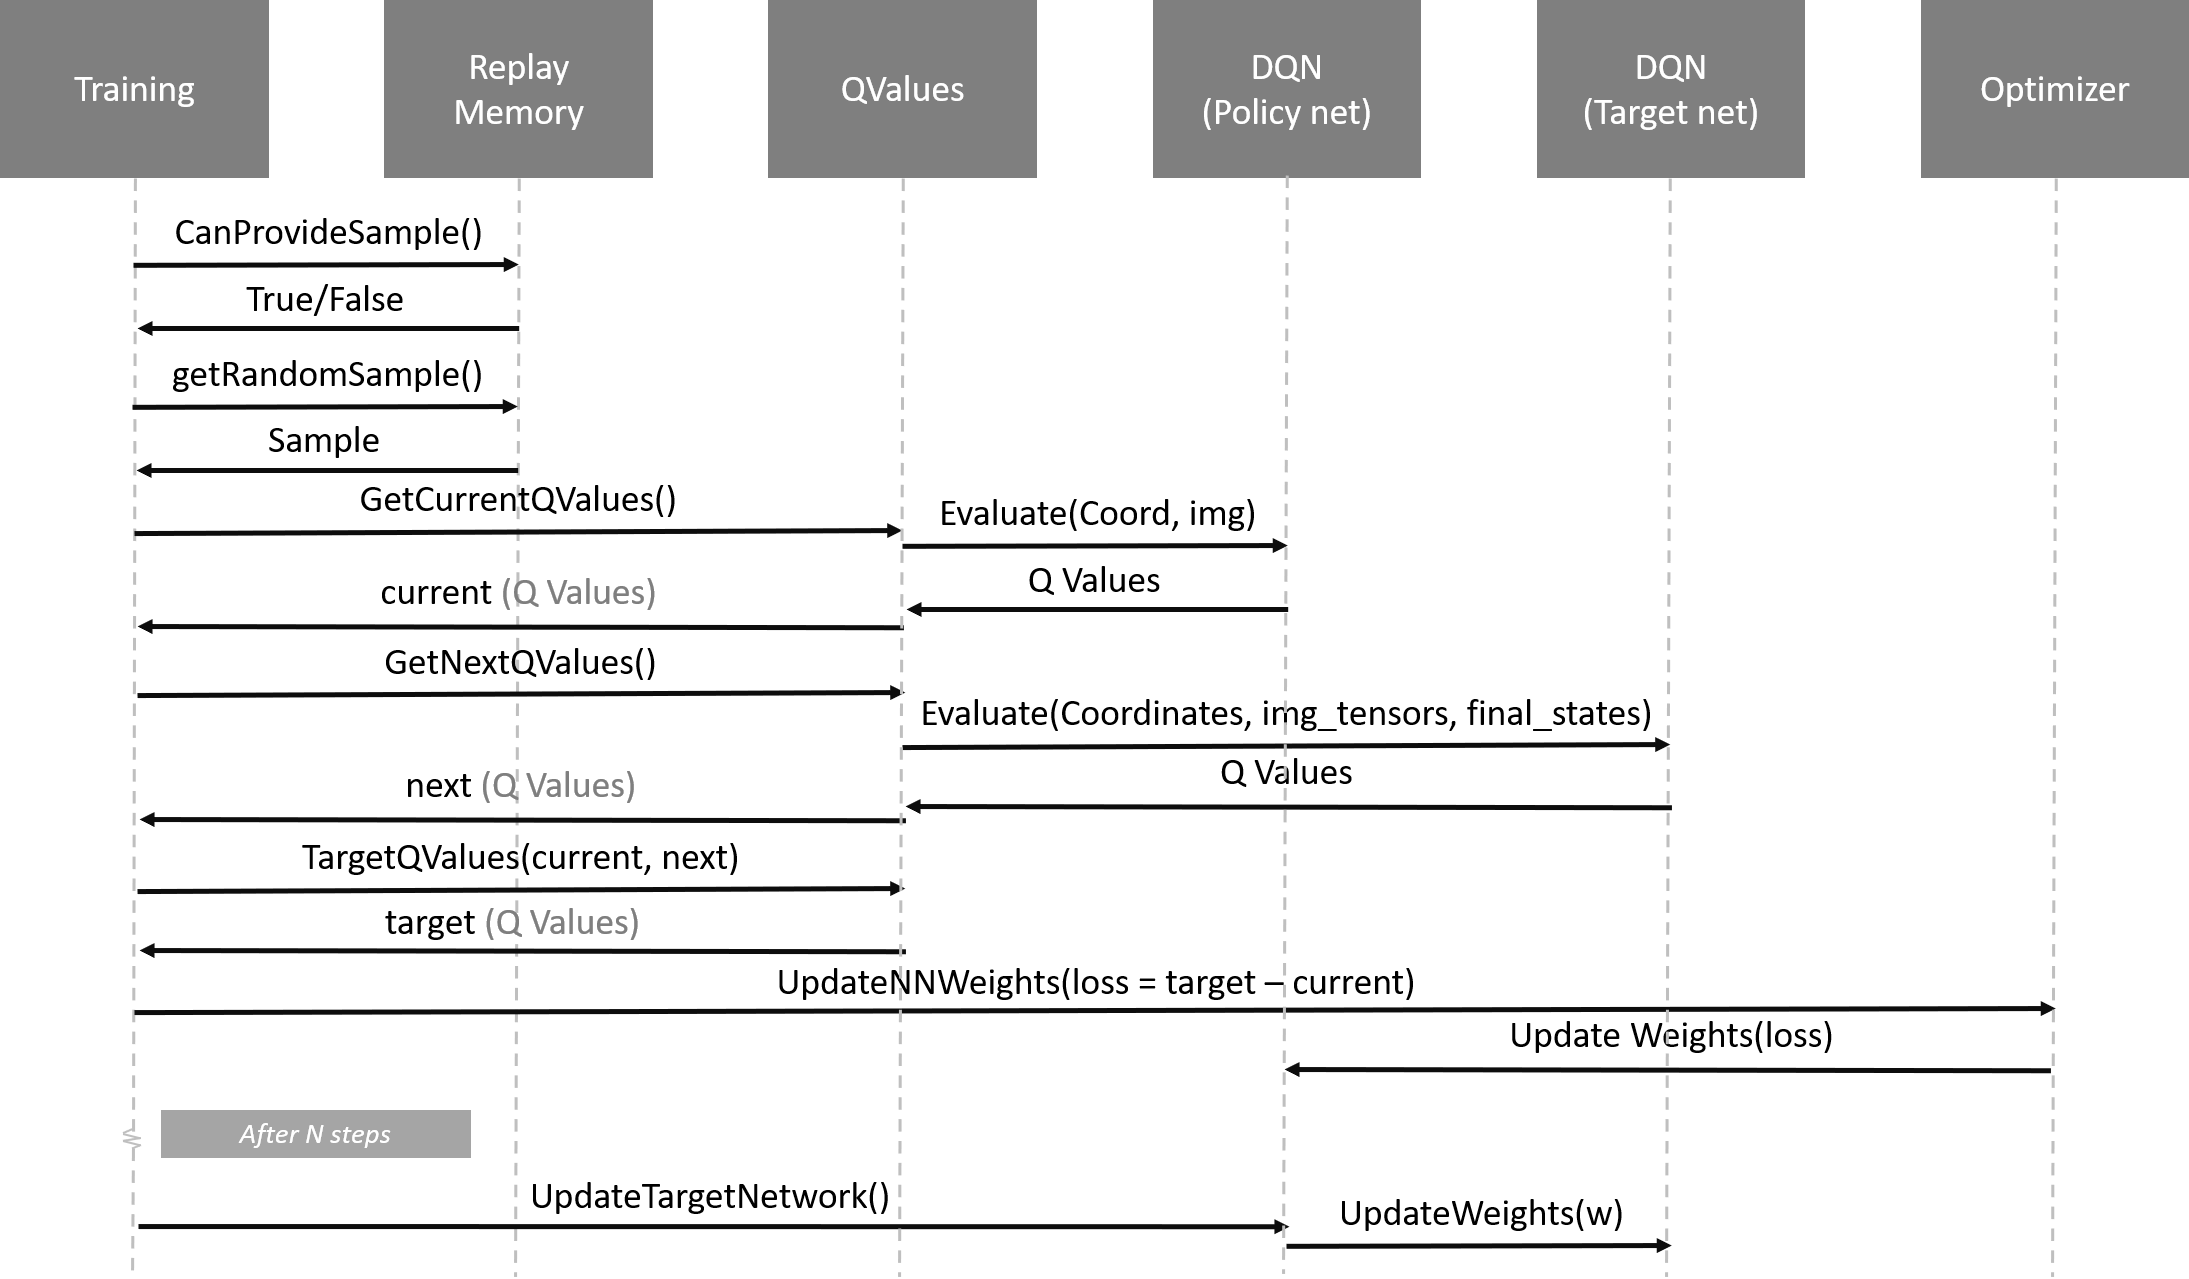
\includegraphics[width=1\linewidth]{Images/TrainingProcess}
					\caption[Training Process]{Flow chart explaining the training process}
					\label{fig:trainingprocess}
				\end{figure}
			
				The training precess starts asking the Replay Memory if there are enough experience to supply a sample of size=batch\_size. If there are enough experience, then the Reply Memory provide a random sample of experiences and the training actually starts. The next step would be splitting the batch into batches of categories and calculate the current and next Q Values of all the samples of the batch.
				
				To calculate the current Q Values we use the policy network and to calculate the next Q values we use the target network. To understand why we use different networks it is recommended to read and try to understand the Deep Reinforcement Learning Section of the State of the Art of this document.
				
				The process of calculating the Q Values is also a little bit different in both cases, because for the next Q Value we have to first take out (Q Value = 0) all the samples of the batch in which the final state is terminal.
				
				Once we have the next Q Values calculated, we use the Bellman's Equation to calculate the target Q Values and then calculate the loss as the difference between the target Q Values and the current Q Values.
				
				Finally, we back-propagate the loss using the optimizer, to modify the weights of the policy neural network. The weights of the target neural network are frozen and only updated after X steps.
				
		\subsection{Image Model}
		
			Image model is the module which is connected to AI Manager and is in charge of extracting the features of the images. It uses some Data augmentation techniques to pre process the image, and then it is passed through a Convolutional Neural network to extract its features.
			
			We will talk about this later, but this is a really important step, not only because a good feature extraction is vital for training any neural network, but also because the size reduction of the image allows us to store a huge amount of experiences in the GPU memory without having to discard any of them because of memory problems.
			
			However, we will not analyse this module more deeply because it was not developed by me and for the aim of this document it works just as a Black Box. The author of this module was Pilar Hernandez, that worked together with me in the project.
				
	\section{Robot Controller}
		
		If the AI Manager is the intelligence of the system, if we continue with the human analogy, the Robot Controller would be the body of the system. As we saw in the \autoref{fig:architecture}, the Robot Controller is the central node, most of the nodes communicates with it, so it is a really important node
		
		Anyway, its complexity is much lower than the AI Manager complexity. The most important task of Robot Controller is to define the set of movements of all the actions. Just to remember, the actions are the ones showed in \autoref{fig:actions}, and Robot Controller will use the UR ICAM MoveIt implementation to perform these actions.
		
		\begin{figure}[H]
			\centering
			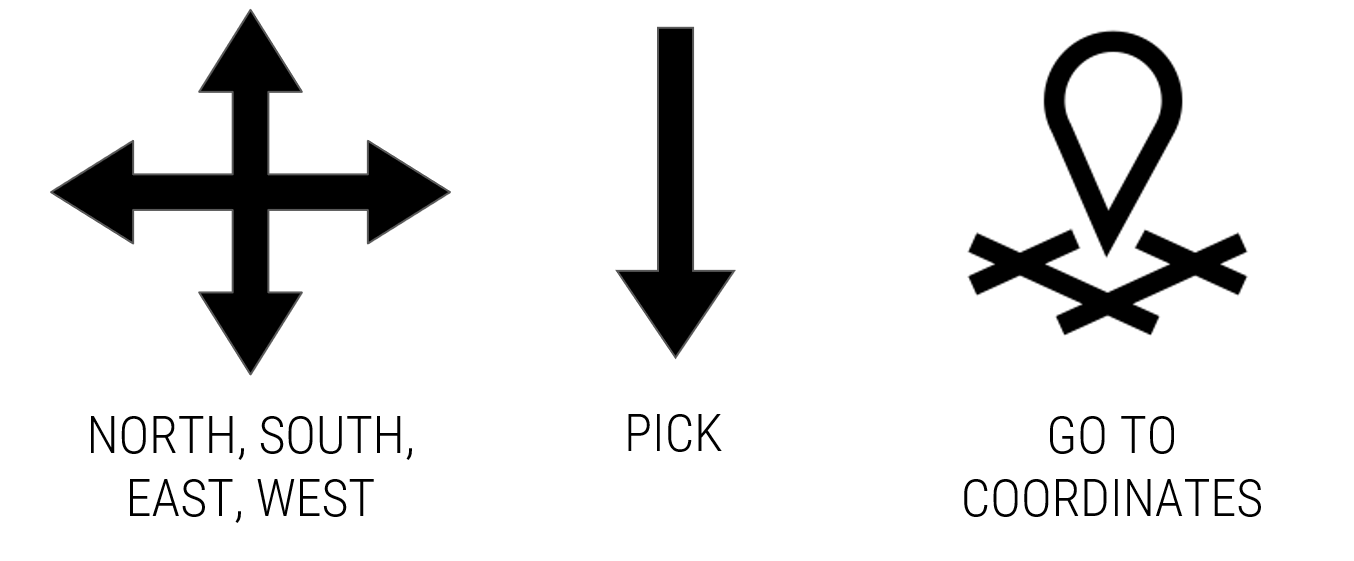
\includegraphics[width=0.9\linewidth]{Images/actions}
			\caption[Actions]{Available actions}
			\label{fig:actions}
		\end{figure}
	
		 With MoveIt, you can tell the robot to go to a specific set of coordinates and it will automatically calculate the best path to reach this position. However, during the implementation of Robot Controller, we found problems executing this kind of movements, because the UR ICAM module wasn't calculating the path correctly, and the robot crashed against itself multiple times. 
		 
		 The solution to this problem was simply stop using this kind of movement, or, at least, to simplify the movement. We realised that we could perform without errors relative movements in every axis, that is to say that we could perform a movement over the axis X, a movement over the axis z but separately, not together. We called this relative move.
		 
		 Let's see how Robot Controller works. In Robot Controller there are multiple files, but only two important files:
		 
		 \begin{itemize}
		 	\item[\textendash]\textbf{\textit{Robot.py}}: In this file we use UR ICAM to implement some methods as relative\_move(x, y, z), and implement all the actions.
		 	\item[\textendash]\textbf{\textit{main.py}}: In this file we basically implement an infinite loop in which asking the service get\_actions for actions and executing them.
		 \end{itemize}
	 
	 	\subsection{Robot.py}
	 	
	 		Robot.py is a python Class that implements a set of methods. It is important to say that Robot.py is also using the Environment.py class that we created in AI Manager, to retrieve all the information about the Environment. We have done it this way to make it easy to change the parameters of training in both AI Manager and Robot Controller at the same time. 
	 		
	 		The methods implemented are:
	 		
	 		\begin{itemize}
	 			\item[\textendash]\textbf{\textit{relative\_move(self, x, y, z)}}: this function takes as parameter the distance in meters to move through each axis. The distance can be positive or negative, and the method will calculate and execute the movements to reach this position.
	 			\item[\textendash]\textbf{\textit{calculate\_relative\_movement(self, relative\_coordinates}}: This method will be used to calculate the relative moves needed to reach certain coordinats. You can see that the parameter passed is called relative\_coordinates. This is like that because we are talking about the coordinates of our environment and not the coordinates of our robot. This make the calculation more difficult, because in UR ICAM we can only get the current Cartesian coordinates of the robot, but not the position of the robot into our environment. 
	 			
	 			To calculate the relative moves needed, though, we will have to translate the relative coordinates on robot coordinates as \textit{Environment.CARTESIAN\_CENTER - relative\_coordinates} and then calculate the difference between the result and the robot current cartesian coordinates.
	 			\item[\textendash]\textbf{\textit{calculate\_current\_coordinates(self)}}: This method is the opposite problem, we use it to translate from robot Cartesian coordinates to Environment coordinates, and we use it to calculate the position of the robot into our environment.
	 			\item[\textendash]\textbf{\textit{take\_north(self, distance=Environment.ACTION\_DISTANCE)}}: This is the north action of the model. It is basically a relative movement of size Environment.ACTION\_DISTANCE in the x axis.
	 			\item[\textendash]\textbf{\textit{take\_south(self, distance=Environment.ACTION\_DISTANCE)}}: This is the south action of the model. It is basically a negative relative movement of size Environment.ACTION\_DISTANCE in the x axis.
	 			\item[\textendash]\textbf{\textit{take\_east(self, distance=Environment.ACTION\_DISTANCE)}}: This is the east action of the model. It is basically a negative relative movement of size Environment.ACTION\_DISTANCE in the y axis.
	 			\item[\textendash]\textbf{\textit{take\_west(self, distance=Environment.ACTION\_DISTANCE)}}: This is the west action of the model. It is basically a relative movement of size Environment.ACTION\_DISTANCE in the y axis.
	 			\item[\textendash]\textbf{\textit{send\_gripper\_message(self, msg, timer=2, n\_msg=10)}}: This is a method used to activate or deactivate the gripper. It sends a burst of messages to ensure that the gripper really switch its state and waits a little bit to allow the robot to pick a piece.
	 			\item[\textendash]\textbf{\textit{take\_pick(self)}}: This is the pick action of the model. To perform this action we have to use a new kind of movement: asynchronous relative movement. It is the same movement than before, but we can execute code during the execution of the movement.
	 			
	 			We need to execute code during the movement because we do not know how far the pieces are, so we have to start going down and, during the execution, check the distance topic in order to know when to stop. Once the robot is in contact with an object, the gripper will send a message to the distance topic, Robot Controller will receive it and will stop the movement. 
	 			
	 			Finally, we activate the gripper using send\_gripper\_message(), will go up to the original position, and will check if the robot has picked an object or not. If it hasn't picked an object it will switch the gripper off and would finish the action, but if it has picked an object, it will execute the take\_place() action.
	 			
	 			To understand better this action, you can check the flow diagram showed in \autoref{fig:nodeinteraction}.
	 			
	 			\item[\textendash]\textbf{\textit{take\_place(self)}}: This is the place action. This is not actually an action of the model, because it theoretically belongs to the pick action, but in the implementation of Robot.py we decided to split the method in two different actions.
	 			
	 			In this action, the robot goes to the place position and then switch the gripper off. In this moment, it take a picture of the environment from the Upper Camera node. Using this picture and the Block Detector analysis, it will calculate the point of the box with a bigger amount of pieces, and will send the coordinates to the take\_random\_state() action.
	 			
	 			\item[\textendash]\textbf{\textit{take\_random\_state(self)}}: This is the action used to reach some coordinates of the box. Probably the name is not the best, if I had to renamed it now I would called it go\_to\_initial\_state(), but at the beginning of the implementation the idea was to make this movement randomly and it took the name from it.
	 			
	 		\end{itemize}
 		
		
		\subsection{Block Detector}
		
			This module is used by Robot Controller but wasn't developed by me, so I will only introduce the goal of the module and what it does, because for the aim of this project it is like a black box. The author of this module was Pilar Hernandez, that worked together with me in the project.
			
			\begin{figure}[H]
				\centering
				\includegraphics[width=0.9\linewidth]{"Images/upper view"}
				\caption[Upper View]{Upper View of the environment}
				\label{fig:upper-view}
			\end{figure}
			
			This module is used during the place action in order to know in which point of the box we should start the next episode. Once the robot had placed the object, it would take a picture from the environment as the one showed in \autoref{fig:upper-view}. Robot Controller would pass the image to the Block detector, which would perform a test similar to the one in \autoref{fig:block-detector}, in which it has calculated all the shapes of the image, and it has calculated the place inside the box with a higher amount of points detected
			
			\begin{figure}[H]
				\centering
				\includegraphics[width=0.9\linewidth]{"Images/Block Detector"}
				\caption[Block Detector]{Block Detector working}
				\label{fig:block-detector}
			\end{figure}
		
			As we can see in the \autoref{fig:block-detector}, where the blue point would represent the return point of the robot, the block detector haven't probably selected the optimal point, but it is a good one, because it is close to a piece when most of the box is empty.
		
	\section{Gripper}
		
		This node is the last one of our architecture. Just to remember, we decided to use a vacuum gripper because it is really easy to pick object with it. Obviously there are objects that you cannot pick with it, but when you can, you just have to push your gripper against the object and activate the pump. The gripper used is the one showed in \autoref{fig:gripper}.
		
		This node is running over an arduino card, which is the controller of the gripper. In the arduino card we have three different peripherals:
		
			\begin{figure}[H]
				\centering
				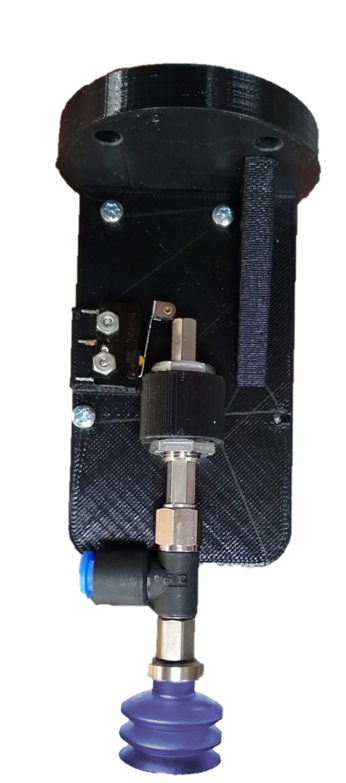
\includegraphics[width=0.7\linewidth]{Images/Gripper}
				\caption[Gripper]{Front view of the gripper}
				\label{fig:gripper}
			\end{figure}
			
			\begin{itemize}
				\item[\textendash]\textbf{Contact sensor:} This is the one that detects if the gripper is in contact with an object. It isn't really a contact sensor, as we can see in \autoref{fig:gripper}, the sucker has actually a mechanical system that can go down or up about 1cm. When a robot touches an object, this object pushes up the sucker and, when the bar goes up it pushes a switch, which is actually the sensor.
				
				It was really difficult to design and make this system work, but we will talk later about that.
				\item[\textendash]\textbf{Object gripped sensor:} To detect if an object has been gripped or not, we have used an air flow sensor. to make it work we connected it as a ramification of the main air pipe. This way, it will not detect any air flow when there is no object picked (All the air is taken from outside), but when an object is picked, the air flow from the outside will stop, creating a vacuum in the pipes and activating the sensor.
				\item[\textendash]\textbf{Pump switcher:} the pump has to be activated or deactivated programmatically from the arduino card.
			\end{itemize}
		
			As commented before, to read or control these peripherals we have the following topics:
			
			\begin{itemize}
				\item[\textendash]\textbf{\textit{\textbackslash distance: }} The gripper is publishing continuously if the gripper is being pushed up or not. Robot Controller wants this information to know when to stop during the pick movement. The Robot basically goes down while \textbf{\textit{\textbackslash distance}} are "False" and stops when they are "True".
				\item[\textendash]\textbf{\textit{\textbackslash switch\_on\_off: }} The gripper listens to this topic. When it receives a "True" message it switch the gripper on, and when it receives a "False" message it switch the gripper off.
				\item[\textendash]\textbf{\textit{\textbackslash object\_gripped: }} The gripper is publishing continuously if there is an object gripped or not. Robot Controller use this information during the pick action. When this action is finished, robot controller checks if an object has been picked or not by reading from this topic. If an object has been picked it goes to the box to place the object and, if not, it just finishes the pick action and request AI Manager for a new action.
			\end{itemize}
		
	\section{Algorithm and System optimization}
	
		Reaching the final version of the system and the algorithm was a really complex and progressive exercise. It is impossible to narrate here all the decisions that we had to make in the process, but I will try to explain the most importants.
		
		\subsection{Performance}
			
			Deep Reinforcement learning can be a really intense CPU and RAM consumer. In fact, during the firs steps of the training the time betwen two actions were between 3 and 5 seconds. This may not look a lot, but having in mind that a Reinforcement Learning training can have more than 10000 steps, we would loose between 30000 and 50000 seconds just calculating actions (We would have to execute them later). In hours, it would be between 8 and a half hours and 13,8 hours.
			
			We had to solve it, so we tried installing a Nvidia GPU in the computer together with the CUDA drivers. After hours of installation, the results were amazing. We designed a load test to test it and these are the results:
			
			\begin{center}
				\begin{tabular}{cccc}
					\toprule 
					& CPU  & GPU \\ 
					\midrule
					\rowcolor{black!20} raiv2 & 3:53 minutes & 49 minutes \\
					dl & 3:14 minutes & 36:31 minutes \\ 
					\bottomrule
				\end{tabular}
				\captionof{table}{Difference in performance between CPU and GPU trainings}
			\end{center}
			
			In the table we can see the time difference between CPU and GPU and between raiv2 and dl. raiv2 is de development computer and dl the execution one, because have a much better GPU and CPU, as it can be seen in the results. It was important to solve this problem, because if we couldn't, we would have to train the network once in each N steps instead of training it in every step.
			
			Another performance problem of Deep Reinforcement Learning has to be with the Replay Memory. In replay Memory we store all the experiences of the agent in order to take smaller samples of experiences to train the algorithm. The problem comes because all the experiences are stored in the GPU memory and, having in mind that in each experience we are saving 2 images, it was impossible to store more than 2000 experiences.
			
			2000 experiences could be enough for the training, but the highest the Replay Memory size, the better. To solve this problem, we decided to store the features extracted from the images instead of the images themselves. With this solution, we introduce a second limitation which is that we heve to finish the training with the same feature extractor that we started it.
			
			However, this isn't a project because we have this limitation anyway, it wouldn't make sense to use a different feature extractor, because the algorithm has been trained with the first feature extractor.
		
		\subsection{Training}
			
			One of the most difficult things in Deep Learning Algorithms is tuning the algorithm. In this case we had to tune two neural networks and the Reinforcement Learning Algorithm. The CNN was training using the images of previous trainings. We performed several days of training with a silly Neural Network. As Reinforcement Learning training it was totally useless, but we used to store and classify thousands of pick images.
			
			The initial image state of every pick action performed was saved together with the success or failure information of the movement. Whith this images and the labels we trained a Neural Network to classify this images, and we used the first layers of this model as feature extractor for the Reinforcement Learning Algorithm.
			
			Then, we had to tune the Reinforcement Learning Algorithm, but we will talk about this in the analysis and results section of this document.
			
		\subsection{Why to use Block Detector?}

			During the first steps of the training, we were doing normal training and, every time that an episode was ended, either by reaching the environment limits or by picking a piece, the robot was starting a new episode by going to a new random pair of coordinates. This looked as the best option at the beginning, because it was the simplest solution, and also because we wanted to ensure low correlation between consecutive steps and random decisions are sometimes the best way of reaching low correlation between samples.
			
			However, during these first episodes we observed that the robot was emptying the pieces of the centre of the box, but it was more difficult for it to pick the pieces that were near to the edges. The coordinates were chosen completely randomly, so we then realized that, although the coordinates probability distribution of the starting point of the episode was uniform, the probability of passing through the centre of the environment during an episode was actually higher than the probability of reaching the box sides. 
			
			The explanation of this is simple, when the initial point of the Episode is in the centre, the probability of reaching any of the four sides of the box is the same while, when the initial point of the environment is one of the sides, its much more complicated to reach another side of the box without passing through the centre.
			
			To check this theory we included the coordinates of ech step in the training statistics, an the results were the ones showed in \autoref{fig:robot-heatmapi}. In this image we can see the heatmap of the movements of the robot and how the probability of reaching the centre of the box was mucho more higher than the probability of reaching the sides.
			
			\begin{figure}[H]
				\centering
				\includegraphics[width=0.9\linewidth]{"Images/Robot HeatmapI"}
				\caption[Robot Heatmap]{Robot position Heatmap}
				\label{fig:robot-heatmapi}
			\end{figure}
		
			In an ideal algorithm, this distribution should be uniform, because the distribution of pieces in the box is uniform. To solve this problem, we used a new strategy for calculating the initial point of the environments. In this case, we decided not to send the robot to de centre of the box, that is to say, sending it always to the sides. With this strategy, we knew that the robot was going to pass through the centre of the box, but we was not expecting the distribution of probabilities to be as uniform as it was. The results were really good, as can be seen in the \autoref{fig:robot-heatmapii}
		
			\begin{figure}[H]
				\centering
				\includegraphics[width=0.9\linewidth]{"Images/Robot HeatmapII"}
				\caption[Heatmap robot II]{Robot position Heatmap with the new strategy}
				\label{fig:robot-heatmapii}
			\end{figure}
		
			The robot behaved better with this new strategy, because now it was managing to empty better the sides of the box. However, there was another problem that we had with both strategies. The problem was that, when the box was almost empty, as the initial position of each episode was chosen randomly, most of the times the robot was going to places with no pieces, and it was taking a lot of time to empty the full box. The robot was working correctly with the box full of pieces, but not were there were just few of them.
			
			To solve this problem, we decided to implement the Block Detector. We commented it before, so I will not explain again how it works, but the important thing is that it allowed us to move the robot to the places with highest amount of pieces, making the robot performance great with or without a high amount of pieces. The best thing is that, as the place with highest amount of pieces varies during the training, the distribution of the robot position kept constantly distributed during the whole box.
			
		\todo{rewards}
		
		\todo{gripper design}
		
		\todo{prior-knowledge}
		
			
			
				
				
			
				 % Developed System
	\chapter{Results Analysis}
	Destacar los resultados más relevantes del proyecto y hacer un análisis crítico de los mismos. También es un capítulo obligatorio y clave.
 % Results Analysis
	\chapter{Conclusions and Future Work}
	Comentar las conclusiones del proyecto, destacando lo que se ha hecho, dejando claros qué objetivos se han cubierto y cuáles son las aportaciones hechas.  % Conclusions and Future Work	

	

	
	%% Include more chapters and or documents.
	
	
	\appendix
		
	\section{Robot Controller}
		En esta sección se muestra el código de algunos de los principales elementos del módulo Robot Controller, implementado en la arquitectura del proyecto.
		
		Este código también está disponible en el siguiente repositorio de github:  
		
		\href{https://github.com/pabloiglesia/robot_controller}{https://github.com/pabloiglesia/robot\_controller}
		\subsection{main.py}
			\lstinputlisting[
			language=Python, 
			% firstline=37, 
			% lastline=45
			]{D:/Proyectos/robot_controller/src/main.py}
	
		\subsection{Robot.py}
			\lstinputlisting[
			language=Python, 
			% firstline=37, 
			% lastline=45
			]{D:/Proyectos/robot_controller/src/Robot.py}
			
			
	\section{Artificial Intelligence Manager}
		En esta sección se muestra el código de algunos de los principales elementos del módulo AI Manager, implementado en la arquitectura del proyecto.
		
		Este código también está disponible en el siguiente repositorio de github: 
		
		\href{https://github.com/pabloiglesia/ai_manager}{https://github.com/pabloiglesia/ai\_manager}
			
		\subsection{main.py}
			\lstinputlisting[
			language=Python, 
			% firstline=37, 
			% lastline=45
			]{D:/Proyectos/ai_manager/src/ai_manager/main.py}
			
		\subsection{RLAlgorithm.py}
			\lstinputlisting[
			language=Python, 
			% firstline=37, 
			% lastline=45
			]{D:/Proyectos/ai_manager/src/ai_manager/RLAlgorithm.py}
	
		\subsection{Environment.py}
			\lstinputlisting[
			language=Python, 
			% firstline=37, 
			% lastline=45
			]{D:/Proyectos/ai_manager/src/ai_manager/Environment.py}
			
		\subsection{ImageController.py}
			\lstinputlisting[
			language=Python, 
			% firstline=37, 
			% lastline=45
			]{D:/Proyectos/ai_manager/src/ai_manager/ImageController.py}
			
			 % Anexos
	
	%% Include appendixes
	
	\cleardoublepage
	
	\printbibliography[heading=bibintoc] % We print the entire bibliography of the document. The author recommends that, if the document contains tremendous amounts of references, that they should be written at the end of each chapter. Refer to https://www.overleaf.com/learn/latex/Bibliography_management_in_LaTeX for more information.
	
	
\end{document}
